\documentclass[a4paper, 12pt]{article}
\usepackage[utf8]{inputenc}
\usepackage{newpxtext, newpxmath}
\usepackage[breaklinks=true]{hyperref}
\usepackage{graphicx}
\usepackage{caption}
\usepackage[left=3cm, right=2cm, top=3cm, bottom=2cm]{geometry}
\geometry{a4paper}
\usepackage{fancyhdr}
\usepackage[brazilian]{babel}
\usepackage{siunitx}
\usepackage{float}
\pagestyle{fancy}
\renewcommand{\headrulewidth}{0pt} 
\lhead{}\chead{}\rhead{}
\lfoot{}\cfoot{\thepage}\rfoot{}
\graphicspath{{../figures/}}
\sisetup{output-decimal-marker={.}}
\usepackage{amsfonts}
\usepackage{mathtools}
\usepackage{cleveref}
\usepackage{spverbatim}
\usepackage{setspace}
\usepackage{subcaption}
\usepackage{csquotes}
\usepackage{booktabs}
\usepackage{pbox}
\setlength{\parskip}{1em}
\singlespacing

\newcommand{\empt}[2]{$#1^{\langle #2 \rangle}$}
\newcommand{\sigmoid}{\text{Sigmoid}}
\newcommand{\sen}{\text{sen}}

\usepackage{amsmath}
\usepackage{enumitem}
\usepackage{tikz}
\usetikzlibrary{shapes,arrows,fit, positioning, arrows.meta}
\usetikzlibrary{backgrounds}
\usepgflibrary{shapes.multipart}
\def\layersep{2.5cm}
\def\layersepp{5cm}	

\begin{document}
\begin{titlepage}
\newcommand{\HRule}{\rule{\linewidth}{1.5mm}}
	
\center


\includegraphics[width=0.15\textwidth]{logo-unicamp.pdf}\\[1.0cm]

\textsc{\Large Estágio Científico e Tecnológico I - EE015}\\[0.5cm]

\textsc{\large Relatório}\\[1.5cm]

{\Large \bfseries Predição de Séries Temporais Baseada em Redes Neurais Artificiais}\\[2.5cm]

\begin{flushleft}
Submetido à \\ Faculdade de Engenharia Elétrica e Computação (FEEC)\\[1.5cm]

Departamento de Engenharia de Computação e Automação Industrial (DCA)\\
Faculdade de Engenharia Elétrica e de Computação (FEEC)\\
Universidade Estadual de Campinas (UNICAMP)\\
CEP 13083-852, Campinas - SP\\[1.0cm]

Aluno: João Pedro de Oliveira Pagnan\\
Orientador: Prof. Levy Boccato \\[4.5cm]
\end{flushleft}	
	
Campinas, \today

\end{titlepage}

\newpage

\section{Introdução}
A predição de séries temporais é uma das aplicações mais interessantes do tratamento de informação. O desafio de antecipar padrões de comportamento e construir modelos que sejam apropriados para explicar determinados fenômenos da natureza tem importância para a biologia, economia, automação industrial, meteorologia e diversas outras áreas da ciência \cite{box2015time}.

É possível definir uma série temporal como sendo um conjunto de observações de uma grandeza ou fenômeno de interesse tomadas durante um intervalo de tempo. Os sistemas cujas medições formam uma série temporal podem ser originados por processos determinísticos ou estocásticos \cite{box2015time}.

Através da análise e interpretação de uma série temporal, podemos estimar os seus valores futuros, aumentando a informação que podemos obter das observações que já foram realizadas em um sistema.

Na literatura, encontramos diversos tipos de modelos para a  predição de séries temporais, desde métodos clássicos lineares, como o modelo autorregressivo (AR) \cite{box2015time} até métodos não-lineares utilizando, por exemplo, redes neurais artificiais, sendo que dessas se destacam as redes do tipo \textit{Multilayer Perceptron} (MLP) e as redes recorrentes, especialmente a \textit{Long Short-Term Memory} (LSTM)  \cite{connor1994recurrent} e a \textit{Echo State Network} (ESN) \cite{jaeger2007echo}.

Uma classe de sistemas dinâmicos particularmente relevante dentro do contexto de modelagem e predição de séries temporais está ligada à ideia de dinâmica caótica. Diversos fenômenos naturais, como a dinâmica populacional de uma espécie, a dinâmica atmosférica de uma região, ou até mesmo as órbitas de um sistema com três ou mais corpos celestes podem exibir comportamento caótico. Apesar de serem determinísticos (e, portanto, previsíveis), esses sistemas são extremamente sensíveis às condições iniciais \cite{fiedler1994caos}. Isso causa um problema para a predição das séries temporais originadas por eles, pois uma pequena incerteza na medida afetará toda a previsão. 

Tendo em vista o desempenho de modelos não-lineares para previsão de diversas séries temporais \cite{connor1994recurrent}, optamos por estudar a aplicabilidade de redes neurais artificiais à previsão de séries relacionadas a sistemas com dinâmica caótica.

Essa primeira parte do projeto de iniciação científica teve como objetivo estudar a base teórica das redes neurais artificiais e de outros regressores lineares clássicos, assim como estudar os fundamentos de sistemas dinâmicos e de dinâmica caótica. 

O estudo dirigido começou abordando uma revisão de tópicos de probabilidade, teoria da informação e estimação. Em seguida, foi vista a teoria de regressores e classificadores clássicos \cite{hastie2009elements}. Depois disso, o estudo se dirigiu para as redes neurais artificiais MLP e recorrentes \cite{geron2019hands}, para, por fim, concluir o aprendizado de preditores com uma breve exposição dos modelos autorregressivos (AR) e autorregressivos de médias móveis (ARMA) \cite{box2015time}. Com a teoria de predição solidificada, o foco mudou para os fundamentos da teoria de sistemas com dinâmica caótica, utilizando como base as referências \cite{fiedler1994caos} e \cite{attux2001dinamica}.

Iniciamos nossa discussão pela Seção 2, na qual são apresentados alguns conceitos básicos de sistemas dinâmicos, seguidos de uma exposição  sobre sistemas caóticos, evidenciando as particularidades que eles têm em relação aos sistemas dinâmicos convencionais.

Em seguida, na Seção 3, veremos os modelos de predição baseados em redes neurais artificiais, juntamente com uma breve exposição de modelos lineares básicos.

Por fim, na Seção 4 são indicados os próximos passos deste projeto de iniciação científica visando sua conclusão no final do segundo semestre de 2021. 

\section{Sistemas Dinâmicos}
O estudo de sistemas dinâmicos se tornou fundamental para a ciência quando a humanidade começou a desenvolver modelos matemáticos para explicar o mundo em sua volta, utilizando os modelos criados para realizar predições e, de certa forma, saber o que nos espera no futuro.

A teoria de sistemas dinâmicos se mostra útil para a modelagem e análise de diversos  fenômenos físicos, biológicos, químicos, ou equações matemáticas, através do tempo. Nesse caso, o tempo pode ser tanto contínuo, quanto discreto \cite{kluever2020dynamic}.

Os sistemas dinâmicos também podem ser lineares ou não-lineares. Um sistema linear, sendo este a tempo contínuo ou discreto, possui a propriedade da superposição, ou seja, se uma entrada consiste de uma soma ponderada de diversos sinais, então a saída é a superposição das respostas do sistema a cada um desses sinais \cite{oppenheim2014signals}. 

É possível representar essa propriedade através das seguintes relações matemáticas, sendo $y(t)$ a resposta de um sistema a tempo contínuo a uma entrada $x(t)$ e $y_i(t)$ a saída correspondente a $x_i(t)$:
\begin{subequations}
\begin{equation}\label{eq:linear-eq-1}
\text{A resposta a } x_1(t) + x_2(t) \text{ é } y_1(t) + y_2(t)
\end{equation}
\begin{equation}\label{eq:linear-eq-2}
\text{A resposta a } a\cdot x_1(t) \text{ é } a\cdot y_1(t)\text{, em que } a \text{ é qualquer constante complexa.}
\end{equation}
\end{subequations}

A primeira equação (\ref{eq:linear-eq-1}) representa a propriedade da aditividade, enquanto a segunda (\ref{eq:linear-eq-2}) representa a propriedade da homogeneidade. Essa definição também é válida para sistemas a tempo discreto, e podem ser combinadas:
\begin{subequations}
\begin{equation}
a \cdot x_1(t) + b \cdot x_2(t) \rightarrow a \cdot y_1(t) + b \cdot y_2(t)
\end{equation}
\begin{equation}
a \cdot x_1[n] + b \cdot x_2[n] \rightarrow a \cdot y_1[n] + b \cdot y_2[n]\mathtt{,}
\end{equation}
\end{subequations}
sendo $a$ e $b$ constantes complexas quaisquer \cite{oppenheim2014signals}.

Devido a todo arcabouço teórico de álgebra linear elaborado por matemáticos nos últimos séculos, trabalhar com modelos lineares de sistemas dinâmicos se tornou algo bem estabelecido. Logo, grande parte dos cursos de graduação lidam,  predominantemente, com sistemas lineares por definição, ou aplicam métodos de linearização em sistemas não-lineares, chegando em soluções analíticas lineares aproximadas, com um bom grau de acurácia sob certas condições de contorno \cite{fiedler1994caos}. 

Com essas aproximações, prever o valor futuro de uma série temporal originada por um sistema linear (ou um sistema não-linear linearizado) é algo relativamente simples, afinal, pode-se utilizar a solução analítica.

Porém, a esmagadora maioria dos fenômenos que observamos na natureza é altamente não-linear. Dessa forma, ou não conseguimos aplicar os métodos de linearização que tanto aprendemos ou, ao serem aplicados, o sistema se reduz a uma representação bem imprecisa da sua dinâmica original \cite{gleick1998chaos}.

Antes de falarmos sobre a teoria da dinâmica caótica, que trouxe diversas explicações para sistemas não-lineares e aumentou o entendimento da ciência sobre esses fenômenos, veremos um pouco sobre alguns conceitos fundamentais no estudo de sistemas dinâmicos.

\subsection{Espaço de Fase}
Algo comum no estudo de sistemas dinâmicos é a representação em espaço de fase (também chamado de espaço de estado). Os eixos do espaço de fase representam os graus de liberdade de um sistema dinâmico. Assim, cada ponto no espaço de fase representa um estado possível para o sistema.

Por exemplo, o movimento de um pêndulo simples, sendo $\theta$ o ângulo entre o pêndulo e o eixo vertical, $g$ a aceleração gravitacional, e $l$ o comprimento do pêndulo, é descrito pela seguinte equação diferencial:
\begin{equation}\label{eq:pendulum}
m l^2 \cdot \ddot{\theta}(t) + mgl\cdot  \sen(\theta(t)) = 0
\end{equation}

Apesar de não ser possível obter uma solução analítica sem antes realizar algum tipo de linearização, é possível estudar a evolução temporal desse sistema através do seu espaço de fases \cite{fiedler1994caos}.

Para tal, escreveremos (\ref{eq:pendulum}) da seguinte forma:
\begin{subequations}
\begin{equation}\label{eq:pendulum-2}
\dot{\theta} = \varphi = f(\theta, \varphi)
\end{equation}
\begin{equation}\label{eq:pendulum-3}
\dot{\varphi} = -\frac{g}{l} \cdot \sen(\theta) = g(\theta, \varphi)
\end{equation}
\end{subequations}

Derivando a equação (\ref{eq:pendulum-3}) em $\theta$ e isolando os termos $\theta$ e $\varphi$ em lados opostos:
\begin{equation}\label{eq:pendulum-4}
\varphi \, d\varphi = -\frac{g}{l} \cdot \sen(\theta) \, d\theta
\end{equation}

Agora, integrando (\ref{eq:pendulum-4}) em ambos os lados, chega-se a:
\begin{equation}
\varphi^2 - \frac{2g}{l} \cdot \cos(\theta) = C
\end{equation}
sendo $C$ uma constante arbitrária. A Figura \ref{fig:pendulum-phase-space} mostra a trajetória no espaço de fases para diversos valores de $C$ (lembrando que $\varphi = \dot{\theta}$).
\begin{figure}[!ht]
\centering
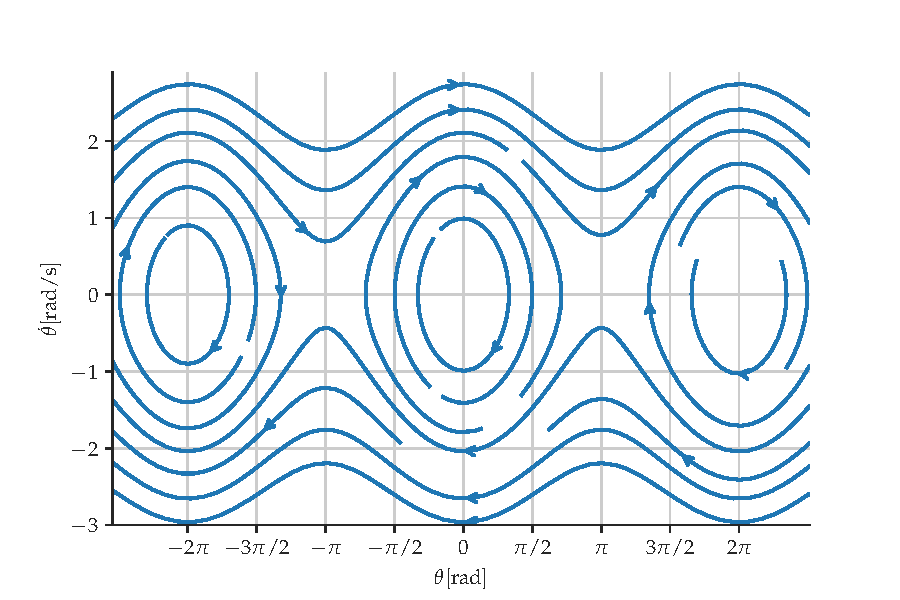
\includegraphics[scale = 0.7]{pendulum-phase-space.pdf}
\caption{Trajetória no espaço de fase do pêndulo simples para vários valores de $C$}
\label{fig:pendulum-phase-space}
\end{figure}

Perceba que um ponto $(\theta, \dot{\theta})$ no espaço de fases representa um estado possível para o sistema. Nesse caso, como não há nenhum elemento estocástico na evolução do pêndulo simples (considerando apenas a mecânica clássica), não há intersecções nas trajetórias no espaço de fases. 

Por fim, é pertinente dizer que o espaço de fases pode ter quantas dimensões forem necessárias para representar a dinâmica de um sistema. 

\subsection{Atratores}
Uma estrutura topológica utilizada para estudar a evolução de um sistema dinâmico, a  qual é capaz de capturar a essência de sua evolução temporal, é o atrator.

De acordo com a definição dada em \cite{fiedler1994caos}, um atrator é um conjunto invariante para o qual órbitas próximas no espaço de fase convergem depois de um tempo suficientemente grande.

Em termos matemáticos \cite{fiedler1994caos}: Uma região compacta $A$ é um atrator de um fluxo $\varphi(t, x)$ se as quatros hipóteses a seguir valem:
\begin{enumerate}[label=\alph*)]
	\item $A$ é invariante segundo $\varphi$;
	\item $A$ tem uma vizinhança contraente;
	\item o fluxo é recorrente, isto é, trajetórias começando em qualquer subconjunto aberto de $A$ voltam a esse subconjunto para valores de $t$ suficientemente longos;
	\item o fluxo não pode ser decomposto, isto é, $A$ não pode ser dividido em duas partes invariantes não triviais.
\end{enumerate}

O formato do atrator varia bastante de acordo com o sistema em análise. Por exemplo, um circuito RLC autônomo tem um atrator chamado de ponto-fixo. Para evidenciarmos isso, considere que as seguintes equações diferenciais descrevem a dinâmica de um circuito RLC, sendo $i$ a corrente no indutor e $v$ a tensão no capacitor \cite{attux2001dinamica}:
\begin{subequations}
\begin{equation}
\frac{di}{dt} = - \frac{1}{L} \cdot (R\cdot i(t) + v(t))
\end{equation}
\begin{equation}
\frac{dv}{dt} = \frac{i(t)}{C}
\end{equation}
\end{subequations}

Assim, dada uma energia inicial presente no sistema, seja esta em forma de campo elétrico no capacitor, ou campo magnético no indutor, o resistor dissipará a energia armazenada em forma de potência ativa (calor). Considerando as variáveis do espaço de estado como sendo a tensão no capacitor e a corrente do indutor, é fácil perceber que a trajetória vai convergir para o ponto $(0, 0)$, pois a energia será toda dissipada e não haverá mais dinâmica nesse sistema.

A Figura \ref{fig:rlc-phase-space} mostra a evolução de um circuito RLC em série para $v(0) = 1$, $i(0) = 1$ com $R = 1$, $L = 1000$ e $C = 500$:
\begin{figure}[!ht]
\centering
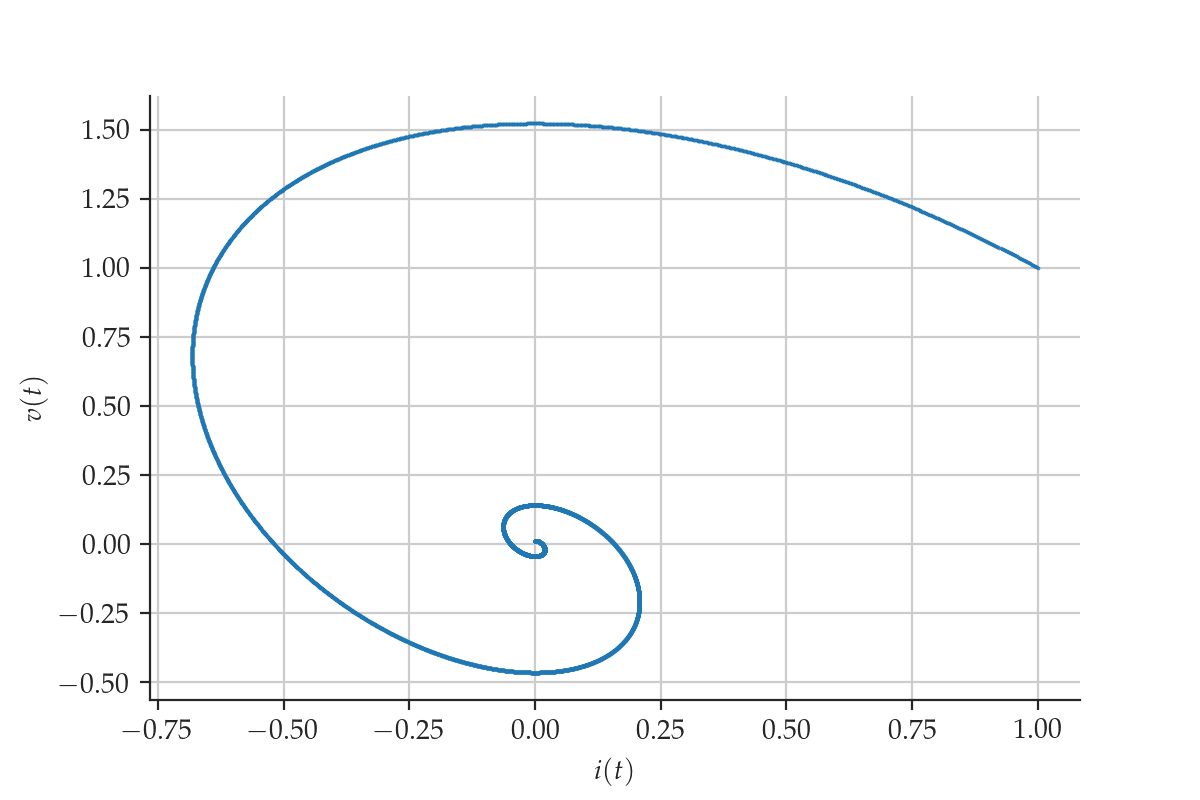
\includegraphics[scale = 0.7]{rlc-phase-space.png}
\caption{Representação do atrator ponto-fixo presente no circuito RLC série}
\label{fig:rlc-phase-space}
\end{figure}

Os atratores podem ser pontos-fixos, ciclo-limites (que é o caso do oscilador harmônico e do pêndulo simples para certos valores iniciais de $\theta$), pontos de nó, pontos de sela, entre outros. Os atratores também podem indicar trajetórias instáveis, estáveis e assintoticamente estáveis. Também é válido mencionar que a região do espaço de fase para a qual todas as trajetórias presentes seguem um determinado  atrator representa a bacia de atração daquele atrator. 

O tipo de atrator e o tipo de estabilidade é obtido analisando os autovalores $\lambda_i$ da representação matricial do sistema dinâmico.

Por fim, quando há uma mudança no sistema dinâmico que faz com que ele seja atraído para a bacia de outro atrator, dizemos que o sistema sofreu uma bifurcação. Geralmente são os parâmetros do sistema que definem os pontos de bifurcação \cite{fiedler1994caos}.

\subsection{Expoentes de Lyapunov}
Considere um sistema contínuo com $m$ equações diferenciais ordinárias, e imagine um pequeno hiper-volume esférico de teste de estados iniciais vizinhos $y_0$ (raio $\varepsilon_0 (x_0)$) em torno do ponto inicial $x_0$ de uma linha de fluxo, isto é \cite{fiedler1994caos}:
\begin{equation}
	|y_0 - x_0| \leq \varepsilon_0 (x_0)
\end{equation}

Com o passar do tempo, o fluxo das trajetórias deforma a hiper-esfera num objeto hiper-elipsoidal com eixos principais $\varepsilon_k (t)$, $k = 1, 2, ..., m$ (Figura \ref{fig:lyapunov}). Os expoentes de Lyapunov medem o crescimento exponencial dos eixos principais $\varepsilon_k (t)$ e são definidos por:
\begin{equation}\label{eq:lyapunov}
\lambda_i = \lim_{t \rightarrow \infty} \lim_{\varepsilon_0 (x_0) \rightarrow 0} \frac{1}{t} \ln \frac{\varepsilon_i (t)}{\varepsilon_0 (x_0)}, \; \; \; i = 1, ..., m.
\end{equation}
\begin{figure}[!ht]
\centering
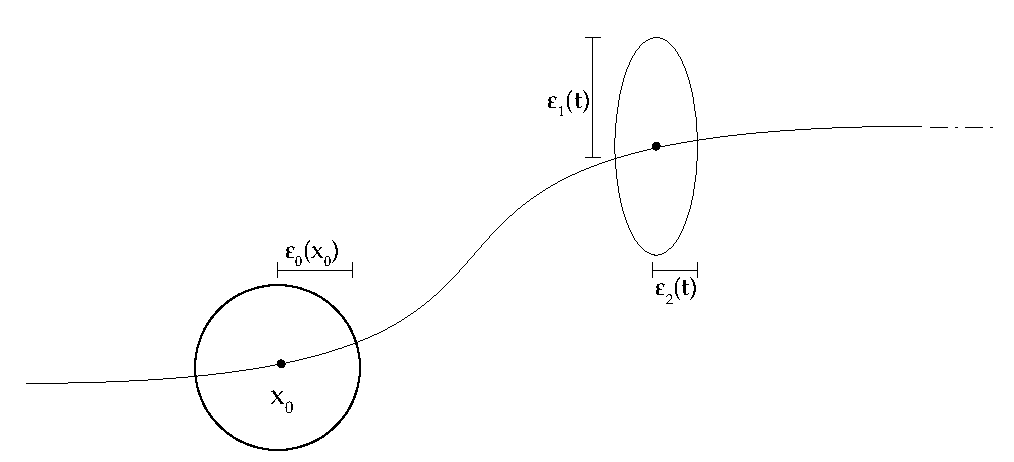
\includegraphics[scale = 0.7]{lyapunov.pdf}
\caption{Evolução de um elemento de volume esférico de raio $\varepsilon_0 (x_0)$ em torno de um ponto inicial $x_0$}
\label{fig:lyapunov}
\end{figure}

A definição em (\ref{eq:lyapunov}) permite a seguinte aproximação:
\begin{equation}\label{eq:lyapunov-approx}
	\varepsilon_i (t) \approx \varepsilon_0 (x_0) \cdot e^{\lambda_i t}
\end{equation}

Da equação (\ref{eq:lyapunov-approx}), conclui-se que \cite{fiedler1994caos}:

a) a existência de um ou mais expoentes de Lyapunov positivos define uma instabilidade orbital nas direções associadas;

b) uma solução caótica tem pelo menos um expoente de Lyapunov positivo (falaremos mais sobre esse fato adiante);

c) uma solução periódica ou quasi-periódica possui $\lambda_i < 0$ nas direções perpendiculares ao movimento no espaço de fase, e $\lambda_i = 0$ ao longo da trajetória.

Agora, considerando que um elemento de hiper-volume $\delta V(t)$ em um instante $t$ é dado por
\begin{equation}\label{eq:lyapunov-volume-1}
\delta V(t) = \prod_{i=1}^{m} \varepsilon_i (t)\mathtt{,}
\end{equation}
tem-se que, substituindo (\ref{eq:lyapunov-volume-1}) em (\ref{eq:lyapunov-approx}):
\begin{equation}
\delta V(t) = \delta V(0) \cdot \exp \big(\sum_{i=1}^{m} \lambda_i t\big)
\end{equation}

A partir dessa definição, é possível concluir que o hiper-volume no espaço de fase não diverge : a) quando $\sum_{i=1}^{m} \lambda_i = 0$, ou seja, quando $\delta V(t) = \delta V(0)$, o que determina um sistema conservativo; b) quando $\sum_{i=1}^{m} \lambda_i < 0$, ou seja, quando $\delta V(t) < \delta V(0)$, o que determina um sistema dissipativo \cite{fiedler1994caos}.

Por fim, é possível identificar o atrator do sistema dinâmico em análise através do sinal dos expoentes de Lyapunov. Por exemplo, no caso tridimensional ($m=3$), caso todos os expoentes $\lambda_i$ sejam negativos, o atrator será um ponto fixo. Já para dois expoentes negativos e um nulo, têm-se um atrator do tipo ciclo-limite.

Os atratores de um sistema caótico possuem uma propriedade especial com relação a seus expoentes de Lyapunov. Esse fato será discutido na Seção 2.5.2.

\subsection{Entropia de Kolmogorov-Sinai}
Também é possível analisar a dinâmica de um sistema através de uma abordagem via teoria da informação.

Para tal, considere um atrator no espaço de estados, recoberto por cubos de lado $\varepsilon$. Agora, seja uma sequência de $b$ cubos $i_1, i_2, ..., i_b$, e seja $p(i_1, i_2, ..., i_b)$ a probabilidade que o sistema se encontre sucessivamente nos cubos $i_1, i_2, ..., i_b$ em intervalos de tempo regulares $\tau$ \cite{fiedler1994caos, attux2001dinamica}. Segundo Shannon  \cite{shannon1948mathematical}, a informação associada à sequência $b$ é proporcional a:
\begin{equation}
I_{b}^{(1)} (\varepsilon) = \sum_{i_1, i_2, ..., i_b} p(i_1, i_2, ..., i_b) \cdot \ln p(i_1, i_2, ..., i_b)
\end{equation}

Perceba que a grandeza:
\begin{equation}\label{eq:shannon-cube-2}
I_{b+1}^{(1)} (\varepsilon) - I_{b}^{(1)} (\varepsilon)
\end{equation}
determina a informação necessária para se localizar o estado do sistema (determinar o cubo $i_{b+1}$ ) sabendo que ele percorreu a sequência de cubos $i_1, i_2, ..., i_b$. A grandeza expressa por (\ref{eq:shannon-cube-2}) quantifica a perda de informação do observador (e o ganho de informação do sistema, consequentemente) entre os instantes de tempo $b \tau$ e $(b+1)\tau$ \cite{attux2001dinamica}.

Com isso, define-se a entropia de Kolmogorov-Sinai como a taxa média de criação de informação no sistema (ou perda de informação do observador) \cite{fiedler1994caos, attux2001dinamica}:
\begin{equation}\label{eq:kolmogorov-sinai}
K = \lim_{\tau \rightarrow 0} \lim_{\varepsilon \rightarrow 0} \lim_{b \rightarrow \infty} \frac{1}{b\tau} \sum_{i_1, i_2, ..., i_b} p(i_1, i_2, ..., i_b) \cdot \ln p(i_1, i_2, ..., i_b)
\end{equation}

A análise da entropia de Kolmogorov-Sinai de um sistema dinâmico revela várias propriedades do comportamento desse sistema ao longo do tempo. Por exemplo, analisando um sistema cuja trajetória segue a bacia de atração de um ponto-fixo, necessitamos de pouca informação para predizer com precisão qual será o estado do sistema em um instante de tempo posterior. Ou seja, não há produção significativa de informação por parte do sistema. Isso também é válido para um sistema cujo atrator é um ciclo-limite.

A entropia de Kolmogorov-Sinai possui uma conexão com os expoentes de Lyapunov. No caso, \cite{attux2001dinamica, fiedler1994caos} mostram que as seguintes equações são válidas, sendo $\lambda_i$ os expoentes de Lyapunov:
\begin{subequations}\label{eq:lyapunov-ksinai}
\begin{equation}
\frac{dI_{i}^{(1)}}{dt} \propto \lambda_i
\end{equation}
\begin{equation}\label{eq:lyapunov-ksinai-entropy}
K \leq \sum_{\lambda_i > 0} \lambda_i
\end{equation}
\end{subequations}

De acordo com a relações em (\ref{eq:lyapunov-ksinai}), podemos concluir que, num sistema determinístico regular (linear e não-linear sem ser caótico ou estocástico), pontos próximos no espaço de fase evoluem sem divergências significativas. Logo, o sistema não produz informação. Assim, a entropia de Kolmogorov-Sinai será nula.

Interessantemente, é visto que, para sistemas estocásticos, a evolução da trajetória no espaço de estado não seguirá nenhum tipo de continuidade, havendo uma perda abrupta de informação por parte do observador. Logo, $K \rightarrow \infty$ \cite{attux2001dinamica}.

Por outro lado, sistemas com dinâmica caótica, apesar de terem uma produção ininterrupta de informação (Seção 2.5.3), têm entropias que seguem a relação dada em  (\ref{eq:lyapunov-ksinai-entropy}). 

Portanto, para vermos mais detalhes do porquê disso ocorrer, na seção a seguir iniciaremos nossa discussão sobre sistemas caóticos.

\subsection{Sistemas com Dinâmica Caótica}
Uma classe de sistemas não-lineares importante para o estudo de diversos fenômenos é a classe de sistemas caóticos. Apesar de ter tido certa dificuldade para encontrar um meio dentro da academia e ser bastante renegada por vários cientistas da época por, entre outros fatores, inicialmente basear-se em simulações  computacionais de dinâmicas físicas, algo que não era comum em meados do século XX \cite{gleick1998chaos}, a teoria da dinâmica caótica foi adotada por cientistas da área da física, matemática, química, biologia, economia, astrofísica, e várias outras, trazendo explicações para diversos fenômenos que não eram bem entendidos até então.

Discutiremos agora algumas propriedades dos sistemas caóticos que os diferem de sistemas lineares e não-lineares convencionais.

\subsubsection{Dimensões fractais no espaço de fase de uma dinâmica caótica}

Como foi dito anteriormente, as trajetórias no espaço de fase de um pêndulo simples não se interseccionam. Isso é devido ao fato de que, como o sistema é determinístico, se ele estiver em um estado $(\theta(t), \dot{\theta}(t))$, só existe um próximo estado possível $(\theta(t + dt), \dot{\theta}(t + dt))$, considerando que é um sistema isolado, sem forças externas. Caso houvesse a intersecção de trajetórias, o sistema teria dois ou mais próximos estados possíveis, o que não é coerente com um sistema determinístico \cite{fiedler1994caos}.

Apesar de apresentar um comportamento errático e, de certa forma, imprevisível, sistemas caóticos são determinísticos. Ou seja, também não há intersecções em suas trajetórias no espaço de fase. Mas, como esses sistemas são capazes de produzir um comportamento tão variado, sem apresentar nenhum tipo de ordem aparente, sem haver intersecções nas trajetórias? Para explicar isso, precisaremos generalizar a noção de dimensão para englobar as dimensões fractais \cite{mandelbrot1967long}. 

O estudo de estruturas topológicas com dimensão fractal tornou-se relevante na matemática nos anos 70 \cite{gleick1998chaos}. Utilizando esse conceito, temos que, além das dimensões inteiras que aprendemos a lidar durante nossa formação (quadrados, cubos, hipercubos etc.), as dimensões fractais representam valores fracionários para essa medida.

Como a base matemática de álgebra linear não engloba essas figuras (pelo menos não no conteúdo que geralmente aprendemos durante a graduação), é necessário o uso de outras ferramentas para estimar a dimensão fracionária. Uma delas é a dimensão de Hausdorff, ou dimensão de Hausdorff-Besicovitch \cite{attux2001dinamica, fiedler1994caos}.

Seja um conjunto de pontos $A$ num espaço de dimensão $N$ e sejam estes pontos recobertos por hiper-cubos de aresta $\varepsilon$. A dimensão de Hausdorff é dada por:
\begin{equation}
D_0 = \lim_{\varepsilon \rightarrow 0} \frac{\log K (\varepsilon)}{\log (1/\varepsilon)}
\end{equation}

Essa definição é válida tanto para figuras de dimensão inteira, como quadrados e cubos, quanto para objetos de dimensão fractal.

Aplicando essa definição numa trajetória no espaço de fase de uma dinâmica caótica, vê-se que a dimensão obtida sempre será fracionária \cite{fiedler1994caos}. Logo, pode-se dizer que a trajetória sofrerá sucessivas contrações em certas direções, e expansões em pelo menos uma, de forma a nunca se cruzar, por mais errático que seja o movimento \cite{fiedler1994caos}.

Uma das propriedades importantes de objetos topológicos de dimensão fractal é que eles apresentam uma auto-similaridade \cite{gleick1998chaos}. Nesse caso, partes da trajetória no espaço de fase têm uma estrutura análoga à da trajetória como um todo \cite{attux2001dinamica}. Ou seja, ao ampliar-se um objeto fractal, suas características serão similares ao do objeto como um todo, tendo uma auto-similaridade.

A Figura \ref{fig:henon} evidencia essa propriedade para o mapa de Hénon \cite{henon1976two}, que é definido pelas seguintes equações a diferenças:
\begin{subequations}
\begin{equation}
x[n+1] = y[n] + 1 - a\cdot (x[n])^2
\end{equation}
\begin{equation}
y[n+1] = b \cdot x[n]
\end{equation}
\end{subequations}
\begin{figure}[!ht]
	\centering
	\begin{subfigure}[b]{0.45\textwidth}
		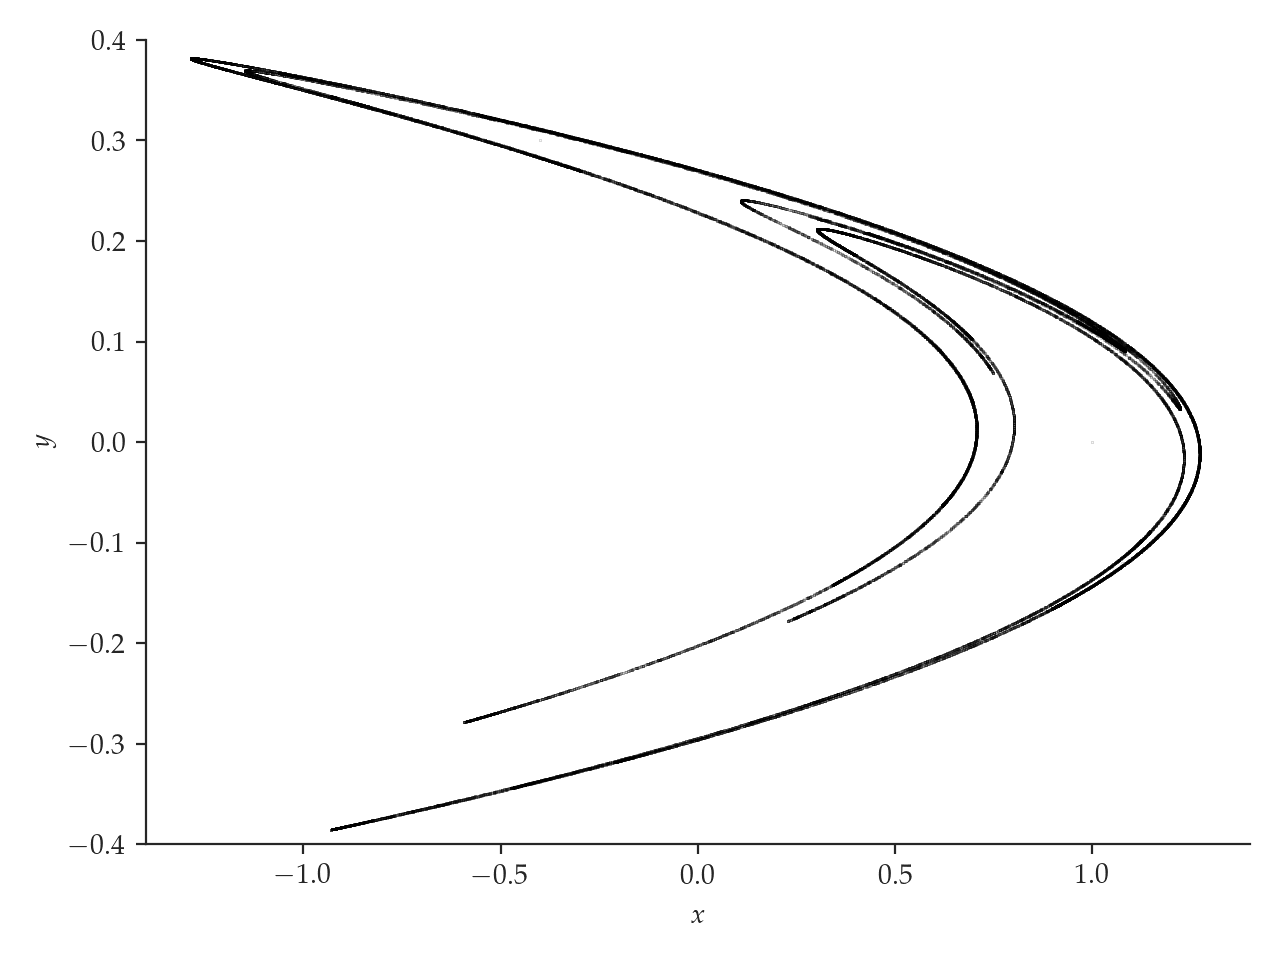
\includegraphics[scale=0.4]{mapa-de-henon.png}
	\end{subfigure}
	\begin{subfigure}[b]{0.45\textwidth}
		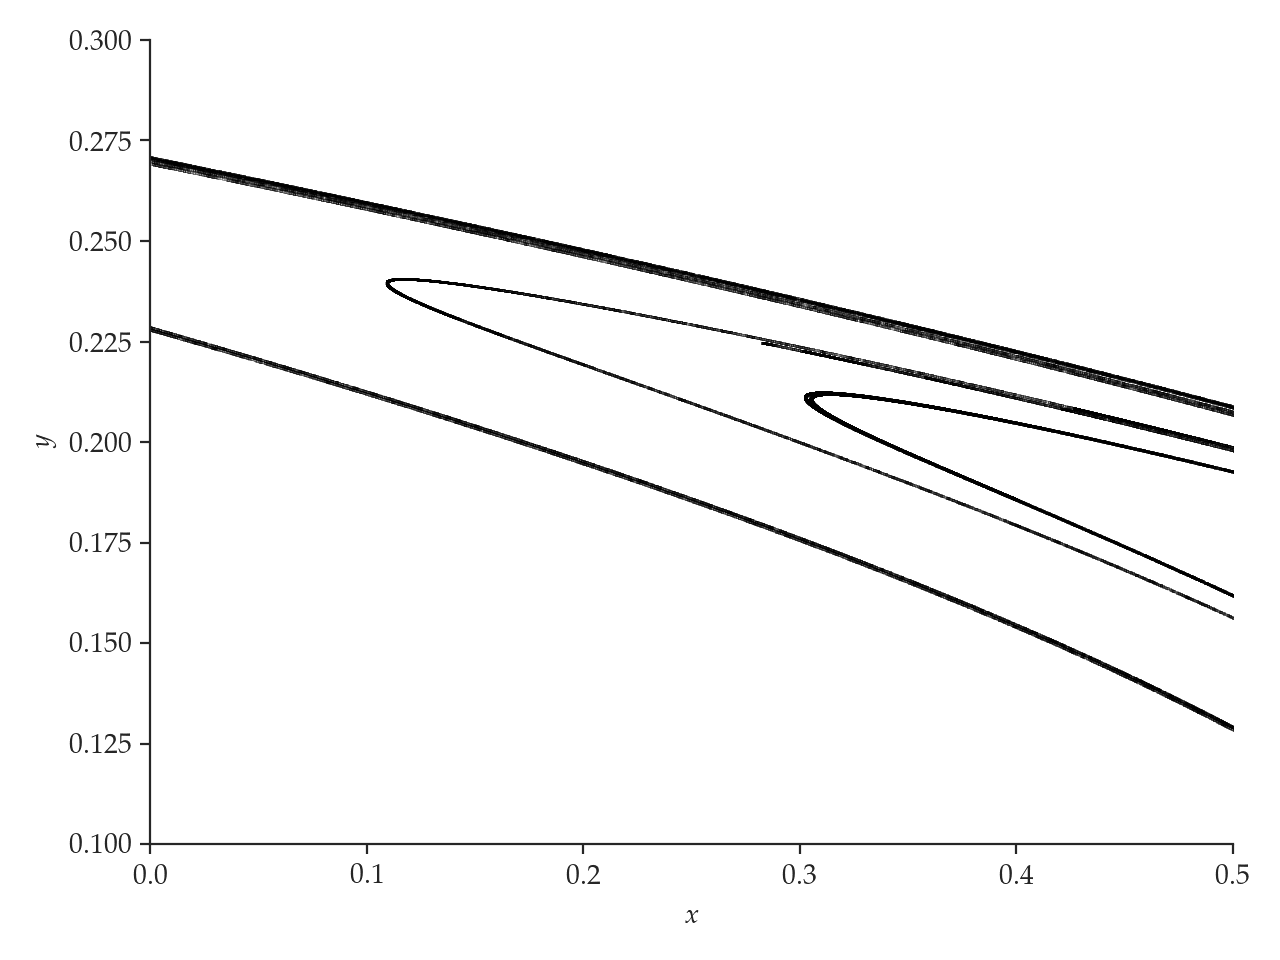
\includegraphics[scale=0.4]{mapa-de-henon-zoom.png}
	\end{subfigure}
	\\
	\begin{subfigure}[b]{0.45\textwidth}
		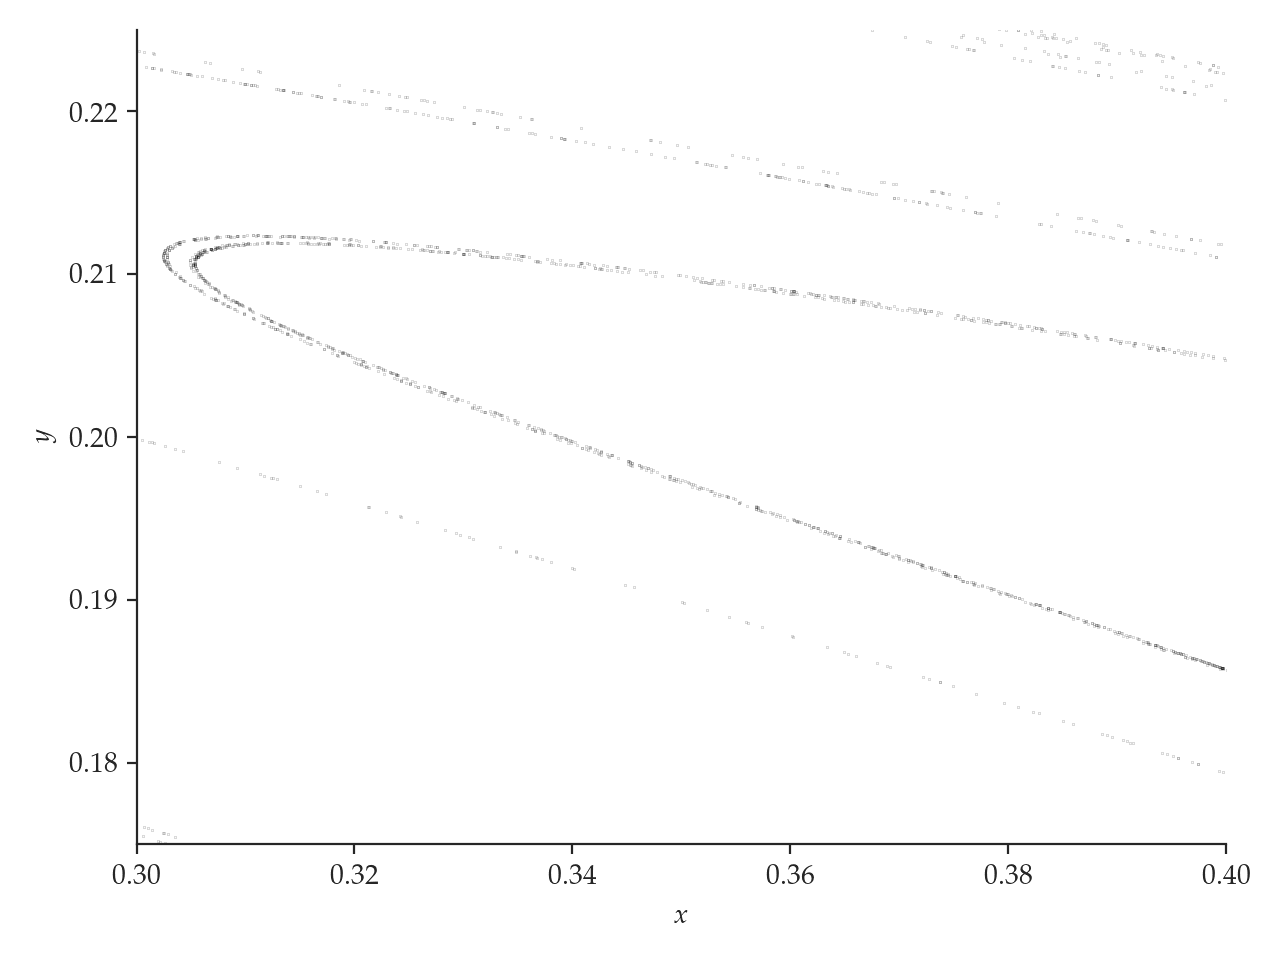
\includegraphics[scale=0.4]{mapa-de-henon-zoom-2.png}
	\end{subfigure}
	\caption{Auto-similaridade presente no mapa de Hénon. Observe o quão similares são as formas observadas nas três figuras, as quais foram obtidas após sucessivas ampliações de trechos específicos nas variáveis $x$ e $y$ no espaço de fase.}
	\label{fig:henon}
\end{figure}

Devido à dimensão fractal e a outros fatores, denominamos os atratores de sistemas caóticos de atratores estranhos \cite{ruelle1971nature}, sendo a própria estrutura presente no mapa de Hénon um atrator estranho. Veremos mais sobre eles na próxima seção.

\subsubsection{Atratores Estranhos}

O termo atrator estranho foi inicialmente cunhado pelos matemáticos David Ruelle e Floris Takens no artigo \cite{ruelle1971nature}, para descrever o fluxo em um fluido turbulento. Esse nome foi dado devido às estranhas propriedades e características dessas estruturas topológicas que as diferenciavam dos atratores convencionais que foram citados na Seção 2.2 \cite{gleick1998chaos}.

De acordo com \cite{attux2001dinamica}, sendo $A$ um conjunto limitado num espaço de $N$ dimensões, dizemos que $A$ é um atrator estranho se for um atrator (utilizando as definições da Seção 2.2) e se, estando a condição inicial $x_0$ num subconjunto de pontos próximos, as evoluções temporais desses pontos apresentarem dependência sensitiva em relação às condições iniciais (DSCI) \cite{fiedler1994caos}.

O ponto que torna esses atratores tão distintos dos usuais é que, no caso linear, espera-se que quando as condições iniciais são próximas, a evolução temporal do sistema no espaço de fase será bem semelhante. A Figura \ref{fig:atrator-rlc-comp} evidencia esse fato para o caso estudado na Seção 2.2, do circuito RLC, onde a diferença entre os estados $(i(t), v(t))$ para as condições iniciais testadas é reduzida com o avanço da simulação.
\begin{figure}[!ht]
\centering
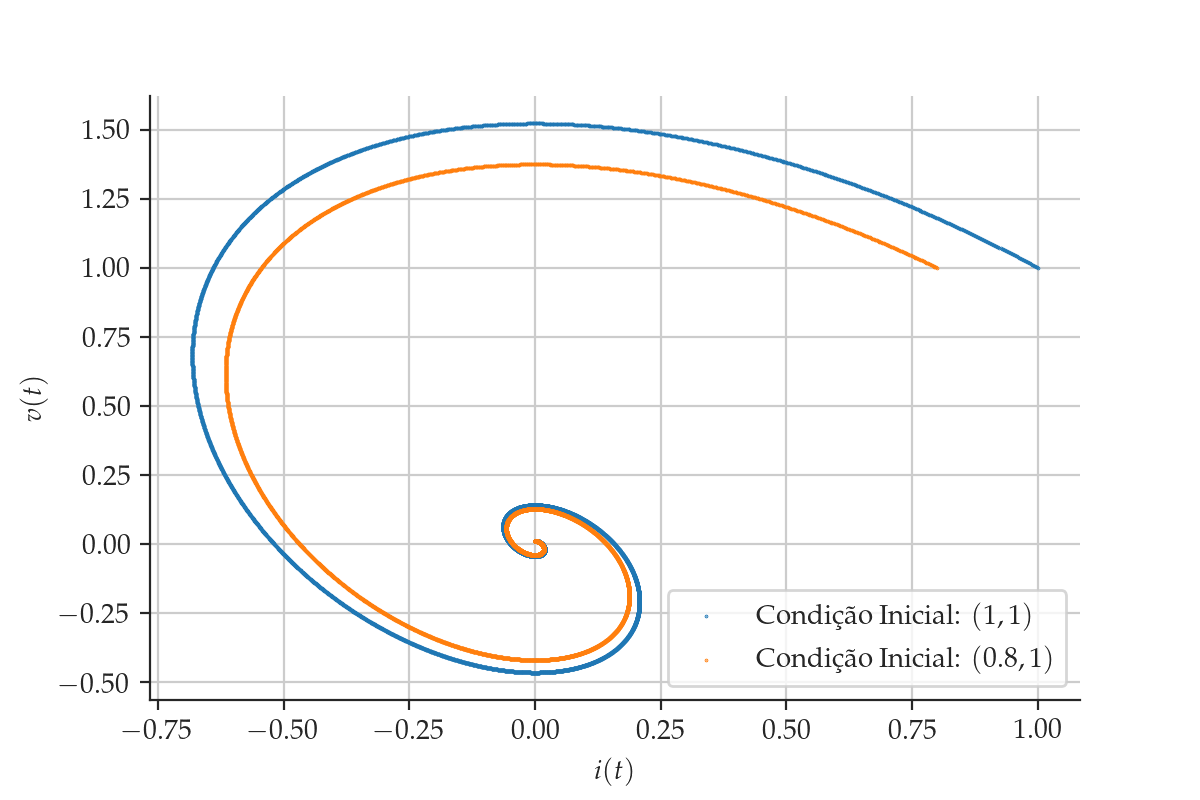
\includegraphics[scale = 0.7]{rlc-phase-space-alt.png}
\caption{Comparação da evolução temporal no espaço de fase de duas condições iniciais próximas no atrator do circuito RLC}
\label{fig:atrator-rlc-comp}
\end{figure}

Para atratores usuais, a diferença entre as trajetórias diminuirá progressivamente (no caso do ponto-fixo), se manterá constante (no caso do ciclo-limite), ou aumentará exponencialmente para o infinito, apresentando uma divergência total.

A característica que torna possível que um atrator estranho apresente comportamentos distintos para condições iniciais próximas, sem divergirem para o infinito, é a dimensão fractal nas trajetórias do espaço de estado, conforme detalhado na Seção 2.5.1. Assim, as sucessivas contrações e expansões do espaço de fase, o que forma uma estrutura fractal, fará com que, por menor que seja a diferença entre as condições iniciais, como há uma infinidade de estados possíveis para a evolução dos mesmos, após algumas iterações do sistema, observaremos que as trajetórias seguiram caminhos distintos entre os estados emaranhados na dimensão fractal.

Além disso, perceba também que as dimensões fractais permitem que haja uma divergência que aumenta exponencialmente, sem divergir para o infinito (o que não ocorre em certos atratores de sistemas que também apresentam divergência). Esse fenômeno é devido ao fato de que as sucessivas expansões e contrações (também chamadas de processo de dobra \cite{fiedler1994caos, attux2001dinamica}) estão contidas em um espaço limitado, devido às dimensões fracionárias (a Seção 2.5.3 apresenta essas características de um ponto de vista da teoria da informação).

Interessantemente, a obrigatoriedade de não haver interseções nas trajetórias no espaço de fases leva à seguinte restrição: sistemas dinâmicos a tempo contínuo devem ter, no mínimo, $3$ dimensões para poderem exibir comportamento caótico, como demonstrado em \cite{guckenheimer2013nonlinear}. Em contrapartida, sistemas dinâmicos discretos com menos dimensões, como o mapa de Hénon (de duas dimensões), já podem ser caóticos. 

Considere o clássico sistema de Lorenz \cite{lorenz1963deterministic}, definido pelas equações diferenciais indicadas abaixo:
\begin{subequations}
\begin{equation}
\frac{dx}{dt} = -\sigma \cdot (x - y)
\end{equation}
\begin{equation}
\frac{dy}{dt} = x \cdot (\rho - z) - y
\end{equation}
\begin{equation}
\frac{dz}{dt} = x \cdot y - \beta \cdot z
\end{equation}
\end{subequations}

A Figura \ref{fig:atrator-lorenz} mostra a evolução temporal do sistema de Lorenz no espaço de fase $(xyz)$ a partir de três condições iniciais próximas.
\begin{figure}[!ht]
\centering
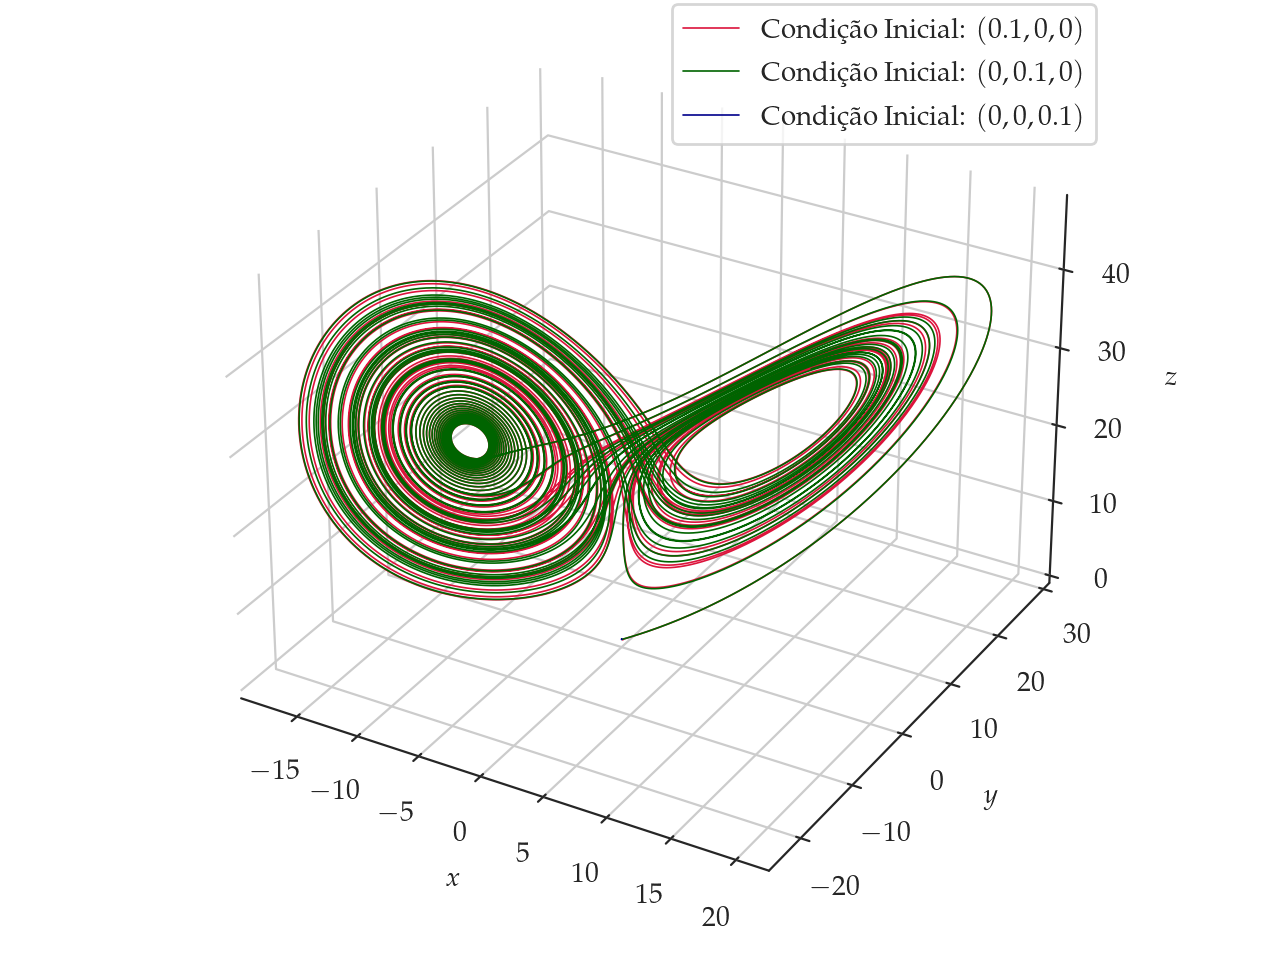
\includegraphics[scale = 0.7]{diagrama-de-fases-alt.png}
\caption{Comparação da evolução temporal no espaço de fase de três condições iniciais próximas para o sistema de Lorenz}
\label{fig:atrator-lorenz}
\end{figure}

A dependência sensitiva em relação às condições iniciais é de tamanha importância para o estudo de sistemas caóticos, que Edward Lorenz, o responsável pelo atrator de Lorenz visto acima, enunciou a seguinte frase na palestra em que pela primeira vez foi apresentado o termo 'efeito borboleta' \cite{gleick1998chaos}:
\begin{displayquote}
"Uma borboleta batendo as asas no Brasil pode causar um tornado no Texas?"
\end{displayquote}

Por fim, como foi mencionado na Seção 2.3, os atratores estranhos possuem uma propriedade interessante com relação aos seus expoentes de Lyapunov. Como foi dito anteriormente na apresentação dos atratores estranhos, as trajetórias no espaço de fase de um sistema caótico possuem uma divergência que é contida em uma região do espaço, sem irem para o infinito (processo de dobra).

Logo, deve haver pelo menos um expoente de Lyapunov positivo. Porém, sistemas caóticos também são dissipativos, ou seja, é válida a relação:
\begin{equation}
\sum_{i=1}^{m} \lambda_i < 0\mathtt{,}
\end{equation}
e, através dessa relação, pode-se provar o fato de que sistemas caóticos em tempo contínuo necessitam de pelo menos $3$ dimensões no espaço de fase. 

Para entender por que essa condição é válida, imagine que seja possível obter um atrator estranho em duas dimensões ($m=2$). Logo, para haver a DSCI, um dos expoentes de Lyapunov é positivo. Porém, uma condição que é válida para toda trajetória no espaço de fase é que, ao longo da direção paralela ao fluxo, o expoente associado é nulo. Então, teríamos um expoente de Lyapunov positivo e outro nulo, o que faria com que $\sum_{i=1}^{2} \lambda_i > 0$, indicando que o elemento de volume divergiria para o infinito, o que não é o caso dos atratores estranhos \cite{fiedler1994caos}. 

Vale mencionar que, apesar dos sistemas caóticos discretos não seguirem essa condição, pode-se mostrar que os mapas (sejam estes uni ou bidimensionais) de seus espaços de estado são amostragens de uma trajetória em três ou mais dimensões, estas sim cumprindo a condição apresentada \cite{fiedler1994caos}.

\subsubsection{Produção de informação em uma dinâmica caótica}

Assim como foi apresentado na seção 2.4, sistemas dinâmicos podem ser estudados analisando a produção de informação através da medida de entropia de Kolmogorov-Sinai.

Para tal, considere as relações em (\ref{eq:lyapunov-ksinai}), que interligam os expoentes de Lyapunov com a produção de informação de um sistema. Consequentemente, quando há pelo menos um expoente de Lyapunov positivo num sistema dinâmico (DSCI), há produção de informação por parte do sistema. Assim, um observador que em $t=0$ tinha uma certa informação sobre o sistema, à medida que o tempo passa sua informação diminui \cite{fiedler1994caos}. 

Porém, como a relação em (\ref{eq:lyapunov-ksinai-entropy}) também é cumprida, a produção segue essa desigualdade. Ou seja, apesar do sistema produzir informação com o passar do tempo, esta não diverge exponencialmente para o infinito (o que caracterizaria um processo estocástico).

Para facilitar a visualização da diferença entre os expoentes de Lyapunov, dimensionalidade e entropia de Kolmogorov-Sinai para os casos de sistemas dinâmicos regulares, sistemas caóticos e sistemas de processos estocásticos, a tabela abaixo sintetiza as informações apresentadas nas últimas seções \cite{fiedler1994caos}:
\begin{table}[!ht]
\begin{center}
\begin{tabular}{c  c  c  c }
  \textbf{Processo}  & \pbox{3cm}{\centering \textbf{Expoentes de\newline Lyapunov}} & \pbox{4cm}{\centering \textbf{\;\, Entropia de\newline Kolmogorov-Sinai}} & \pbox{5cm}{\centering \textbf{\;\, Dimensão da\newline dinâmica assintótica}\newline $(t\rightarrow \infty)$} \\
 \hline
 \textbf{Regular} & $\nexists\;  \lambda_i > 0$ & $K = 0$ & $D < m, \; D\in \mathbb{N}$ \\  
  \addlinespace
 \textbf{Caótico} & $\exists\; \lambda_i > 0$ & $0 < K \leq \sum_{\lambda_i \geq 0} \lambda_i$ & \pbox{5cm}{\centering $D < m, \; D\in \mathbb{R}$ \newline Sistemas contínuos: $m \geq 3$}\\   
  \addlinespace
 \textbf{Estocástico} & --- & $K \rightarrow \infty$ & $D=m$ 
\end{tabular}
\caption{Comparação dos Expoentes de Lyapunov, da Entropia de Kolmogorov-Sinai e da Dimensionalidade para sistemas dinâmicos regulares, caóticos e estocásticos}
\end{center}
\end{table}

\subsubsection{A série temporal e o espectro de potências de um sistema caótico}
Outra abordagem possível para o estudo de sistemas dinâmicos caóticos envolve a análise de suas séries temporais. 

Para isso, uma ferramenta que permite obter conclusões interessantes, podendo indicar a rápida perda de informação por parte do observador, mencionada na seção anterior, é a análise da autocorrelação e da autocorrelação parcial de uma série temporal.

Através de \cite{fiedler1994caos}, pode-se definir a função de autocorrelação $\phi_m$ como a média do produto dos valores de um sinal $x(t)$ em instantes de tempo espaçados de $\Delta t$, indicando por quanto tempo o valor do sinal no instante $t$ depende de seus valores prévios e medindo o grau de semelhança existente no sinal à medida que o tempo passa:
\begin{equation}
\phi_m = \frac{1}{N} \sum_{j=1}^{N} x_j x_{j-m}
\end{equation}

Similarmente, a autocorrelação parcial encontra a correlação dos valores da série $x_j$ e $x_{j-m}$ após o ajuste para remover o efeito da presença dos termos intermediários $x_{j-1}$, $x_{j-2}$, ..., $x_{j-m+1}$.

A Figura \ref{fig:henon-time-series} exibe a série temporal, a autocorrelação e a autocorrelação parcial para um atraso $K$ na série temporal discreta do mapa de Hénon, mencionado anteriormente, associada à variável $x$.
\begin{figure}[!ht]
	\centering
	\begin{subfigure}[b]{0.45\textwidth}
		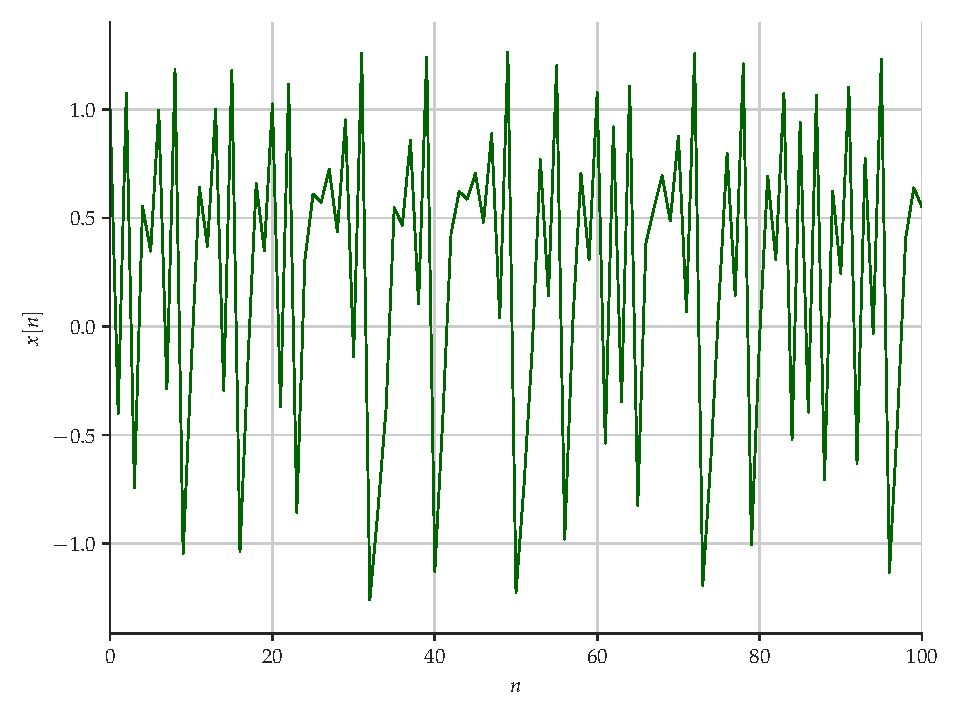
\includegraphics[scale=0.4]{series-temporal-x.pdf}
	\end{subfigure}
	\begin{subfigure}[b]{0.45\textwidth}
		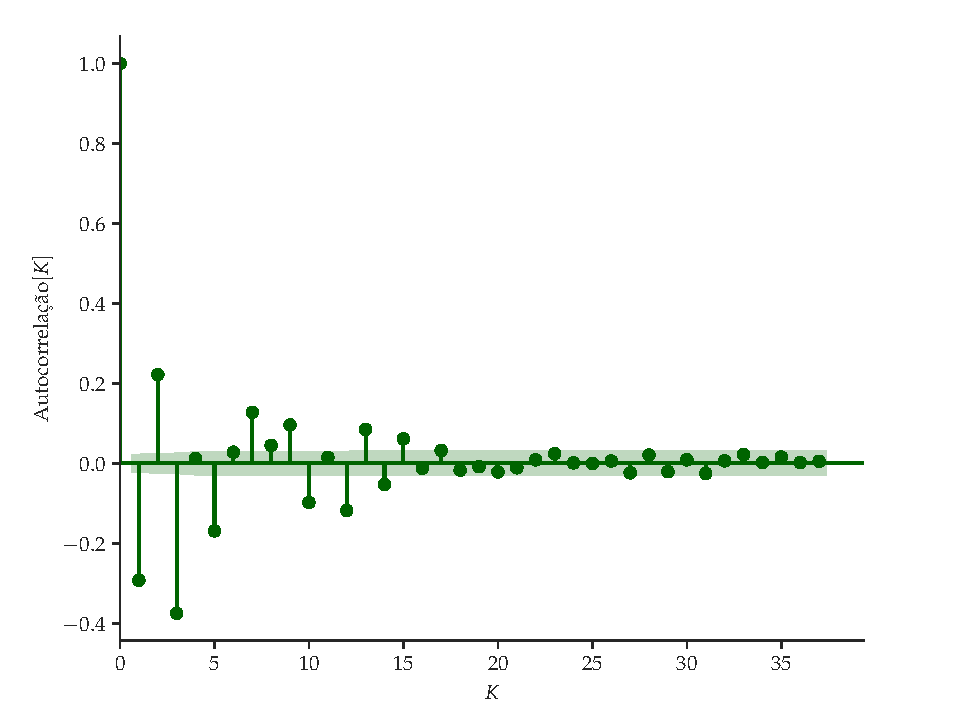
\includegraphics[scale=0.4]{autocorrelacao-henon.pdf}
	\end{subfigure}
	\\
	\begin{subfigure}[b]{0.45\textwidth}
		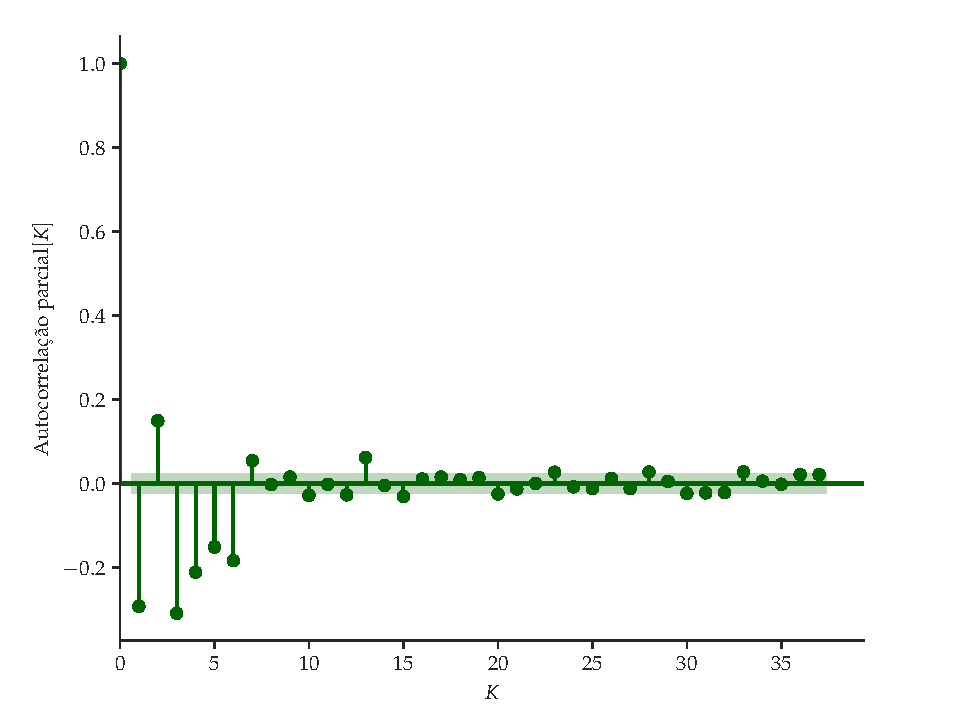
\includegraphics[scale=0.4]{autocorrelacao-parcial-henon.pdf}
	\end{subfigure}
	\caption{Série temporal, autocorrelação, e autocorrelação parcial para o mapa de Hénon em $x$}
	\label{fig:henon-time-series}
\end{figure}

Além do fato que a série temporal é extremamente errática, perceba também que a autocorrelação parcial decai rapidamente, sendo que, a partir de $K = 8$, não há mais uma presença significativa (evidenciado pela faixa verde na figura). Esse fato é importante, pois nos basearemos nestes valores de correlação para estabelecer quantas amostras passadas devem ser fornecidas na entrada dos preditores (falaremos mais sobre isso a partir da Seção 3).

Por fim, o espectro de potências $P(\Omega) = |X(e^{j\Omega})|^2$ do sinal de uma série temporal originada por um sistema caótico também possui propriedades interessantes. A Figura \ref{fig:henon-power-spectrum} mostra esse espectro para a série temporal do mapa de Hénon exibida acima:
\begin{figure}[!ht]
\centering
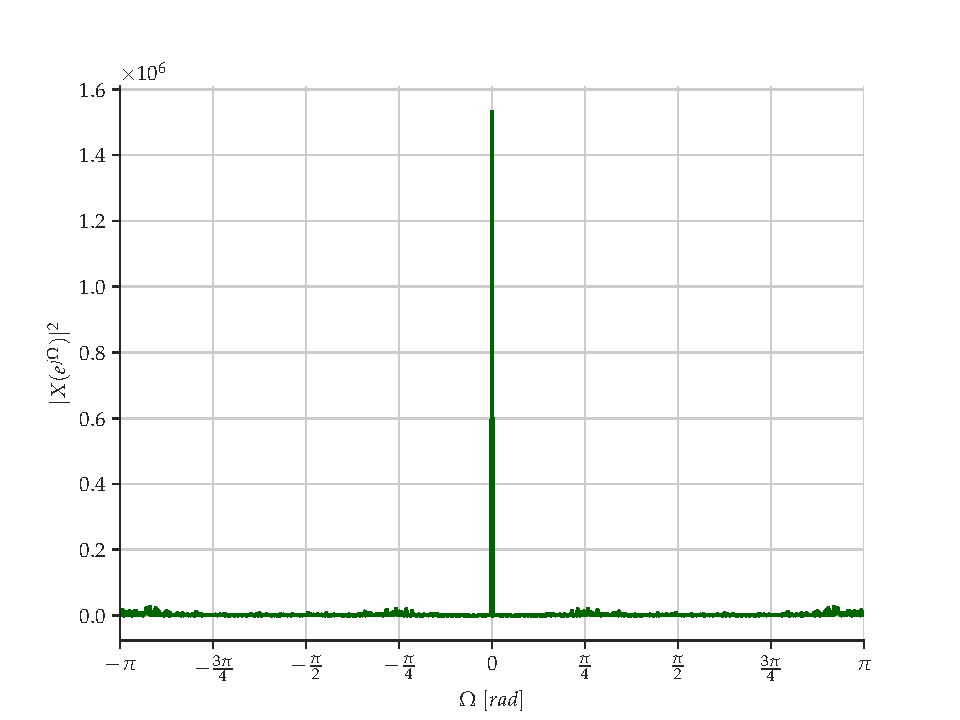
\includegraphics[scale = 0.5]{power-spectrum-henon.pdf}
\caption{Espectro de potências para a série temporal do mapa de Hénon em $x$}
\label{fig:henon-power-spectrum}
\end{figure}

Analisando o espectro, é possível perceber que ele é bem similar a um espectro de uma série temporal de um processo estocástico, sendo contínuo e de faixa larga. Para  descobrir se uma série temporal tem origem em um processo caótico ou estocástico, normalmente são utilizadas técnicas de reconstrução dos atratores desses sistemas \cite{packard1980geometry}, inclusive algumas mais recentes utilizando ferramentas de \textit{machine learning} \cite{lu2018attractor}.

\subsubsection{Características gerais de um sistema com dinâmica caótica}
Depois de uma exposição de alguns conceitos fundamentais de sistemas dinâmicos, além de alguns pontos sobre dinâmica caótica, podemos sintetizar o que foi apresentado nas propriedades fundamentais do caos determinístico em sistemas dinâmicos \cite{attux2001dinamica}:
\begin{enumerate}
\item Forte sensibilidade com respeito às condições iniciais (DSCI);
\item A evolução temporal das variáveis de estado é rápida e tem uma aparência errática;
\item Um sinal originado por um sistema caótico tem espectro de potências contínuo e de faixa larga;
\item Há uma produção de informação por parte do sistema;
\item Presença de atratores estranhos.
\end{enumerate}

Logo, um sistema dinâmico que possui essas propriedades é um sistema caótico.

Nossa análise será sobre a predição das séries temporais originadas por esses sistemas. Por tudo que foi dito até aqui, é esperado que não seja uma tarefa fácil estimar seus valores futuros.

Por causa disso, o estudo se direcionará à aplicabilidade das redes neurais à predição, ou seja, utilizando ferramentas que também são não-lineares, assim como os sistemas em estudo. Logo, na seção a seguir serão discutidos algumas estruturas de redes neurais artificiais, além de uma breve exposição sobre modelos clássicos lineares.

\section{Modelos de Predição}

\subsection{Modelos Lineares}

Apesar desta pesquisa se dedicar à aplicação de modelos de predição não-lineares (mais especificamente, algumas opções de redes neurais artificiais), é pertinente darmos uma introdução ao assunto através de modelos lineares para essa aplicação, já aproveitando o momento para apresentarmos alguns conceitos básicos de predição.

\subsubsection{Modelo Autorregressivo (AR)}

No modelo autorregressivo (AR, do inglês \textit{autoregressive}) o valor da série para um instante de tempo $n$, denotado por $x(n)$, é dado pela combinação linear dos valores passados a partir do instante $n - L - (K - 1)$ até o instante $n - L$, onde $L$ é o passo de predição (quantos instantes de tempo à frente pretende-se predizer o valor da série) e $K$ é a ordem do modelo. 

Portanto, podemos dizer que, no modelo AR o valor da série temporal num instante $n$ é dado por \cite{haykin2008adaptive}:
\begin{equation}
x(n) = a_{1} \cdot x(n - L) + a_{2} \cdot x(n - L - 1) + ... + a_{K} \cdot x(n - L - (K - 1)) + \eta (n)
\end{equation}
onde $a_{k}$, $k = 1, 2, ..., K$ são os coeficientes que ponderam as amostras nos instantes passados e $\eta (n)$ é o erro instantâneo do modelo preditor. Esse erro instantâneo é um ruído branco (do inglês, \textit{white noise}), possuindo média nula e variância $\sigma_{n}^2$ constante \cite{box2015time}.

É interessante mencionar que, se considerarmos $L = 1$, ou seja, se estivermos predizendo o valor da série num instante seguinte ao atual, podemos dizer que:
\begin{equation}\label{ar-l-1}
\sum_{k=0}^{K} w_{k} \cdot x(n - k) = \eta (n)
\end{equation}
sendo $w_{0} = 1$ e $w_{k} = -a_{k}$ para $1 \leq k \leq K$.

Perceba que o lado esquerdo de (\ref{ar-l-1}) é uma soma de convolução em tempo  discreto. Portanto, podemos interpretar o modelo AR como um sistema linear e invariante com o tempo (LIT) \cite{haykin2008adaptive}.

\subsubsection{Modelo Autorregressivo e de Médias Móveis (ARMA)}

O modelo ARMA (do inglês, \textit{auto-regressive moving-average}) incorpora à construção de $x(n)$ valores passados do ruído branco (ou do erro de predição), de forma que \cite{box2015time}:
\begin{equation}
x(n) = \sum_{k = 1}^{K} a_{k} \cdot x(n - L - (k-1)) + \sum_{k=1}^{M} b_{k} \cdot \eta(n - L - (k-1))
\end{equation} 

Dado um conjunto de observações temporais, a construção de um modelo ARMA que aproxime tal conjunto requer o uso de métodos iterativos e/ou heurísticos de otimização. Isso é devido ao fato de que não há soluções em forma fechada para obter os coeficientes $b_k$. Além disso, é válido mencionar que durante a otimização desses parâmetros, devemos nos atentar à estabilidade desse sistema, afinal, os erros podem se acumular, levando a uma divergência na saída do preditor \cite{box2015time}.

Apesar dos modelos lineares ainda serem bastante utilizados para a predição de séries temporais, para determinadas situações a regra linear aplicada pelos modelos AR e ARMA não é suficiente para realizar uma predição com um erro aceitável em sistemas mais complexos. 

Devido a isso, optamos por direcionar o estudo para modelos de predição não-lineares baseados em redes neurais artificiais. Vejamos, então, como são estes preditores. 

\subsection{Modelos Não-lineares}

Os modelos não-lineares estudados foram as famosas redes neurais artificiais.

As redes neurais artificiais são ferramentas computacionais cujas estruturas são inspiradas no funcionamento das redes neurais biológicas presentes em cérebros de animais desenvolvidos, em especial do ser humano. Podemos interpretar um neurônio (tanto biológico, quanto artificial) como uma unidade de processamento de informação \cite{haykin2010neural}. 

Analogamente, uma rede neural artificial é uma estrutura formada por vários neurô\-nios artificiais interconectados, a qual é capaz de processar estímulos (sinais) de entrada e de produzir respostas conforme a tarefa desejada. Existem alguns modelos matemáticos para o neurônio artificial, sendo o \textit{perceptron} um dos mais usuais (vide Seção 3.2.1). Além disso, os neurônios podem ser organizados de diferentes maneiras para construir a arquitetura (ou topologia) da rede neural, a qual é tipicamente estruturada em camadas. Por fim, os neurônios artificiais podem exibir uma estrutura interna que varia de acordo com a arquitetura desejada para a aplicação, como observaremos na Seção 3.2.2, onde são discutidos alguns exemplos de redes recorrentes.

\subsubsection{Redes \textit{Multilayer Perceptron} (MLP)}
Um dos modelos mais utilizados para representar um neurônio artificial, o \textit{Perceptron} \cite{rosenblatt1958perceptron}, é apresentado na Figura \ref{fig:mlp}.
\begin{figure}[H]
\begin{center}
\begin{tikzpicture}[thick,scale=0.7, every node/.style={transform shape}]
	\tikzstyle{rectangle_style}=[rectangle, draw, minimum height = 15mm, minimum width = 12.5mm]
	\tikzstyle{circle_style}=[circle, draw]
	\tikzstyle{dividedrectangle_style}=[draw, rectangle split, rectangle split parts=2, rotate = 90, minimum height = 15mm, minimum width = 10mm]
	
	% neuron i
	\draw node at (-0.33, 0) [] (neuron_i_0) {$x_0 = 1$};
	\foreach \x in {1,...,2}
		\draw node at (0, -1.5*\x) [] (neuron_i_\x) {$x_\x$};
	\foreach \x in {1,...,3}
		\fill (0, -3.5 - 1.5*\x*0.15) circle (1pt);
	\draw node at (0, -5) [] (neuron_i_3) {$x_m$};
	\node at (neuron_i_0.north) [above, inner sep=3mm] {\small \textit{\textit{Entradas}}};			
	
	% w_ji
	\foreach \x in {0,...,2}
		\draw node at (1.5, -1.5*\x) [circle_style] (w_ji_\x) {$w_{\x}$};
	\draw node at (1.5, -5) [circle_style] (w_ji_i) {$w_m$};
	\foreach \x in {1,...,3}
		\fill (1.5, -3.5 - 1.5*\x*0.15) circle (1pt);
	\node at (w_ji_0.north) [right, inner sep=5mm] {\small \textit{\textit{bias}}};	
	\node at (w_ji_i.south) [below, inner sep=3mm] {\small \textit{\textit{Pesos Sinápticos}}};		
	
	% neuron j
	\node at (6.5, -1.5) [circle_style] (neuron_j) {{\Huge $\sum$}};
	\node at (neuron_j.south) [below, inner sep=3mm] {\small \textit{Junção Somadora}};	
	
	% activation
	\node at (9, -1.5) [rectangle_style] (activation) {$\varphi (\cdot)$};
	\node at (activation.north) [above, inner sep=1mm] {\small \textit{Função de Ativação}};
	
	% output
	\node at (12, -1.5) [] (output) {$y$};
	\node at (output.north) [above, inner sep=1mm] {\small \textit{Saída}};	

	% connect: y_i -> w_ji
	\foreach \i in {0,...,2}
		\path[->] (neuron_i_\i) edge node[] {} (w_ji_\i);
	\path[->] (neuron_i_3) edge node[] {} (w_ji_i);
	
	% connect: w_ji -> neuron j
	\foreach \i in {0,...,2}
		\path[->] (w_ji_\i) edge node[] {} (neuron_j);
	\path[->] (w_ji_i) edge node[] {} (neuron_j);
	
	% connect: neuron j -> activation
	\path[->] (neuron_j) edge node[above, midway] {$v$} (activation);
	
	% connect: activation -> output
	\path[->] (activation) edge node[] {} (output);
	
\end{tikzpicture}
\caption{Modelo \textit{Perceptron} para o neurônio artificial}
\label{fig:mlp}
\end{center}
\end{figure}

Em termos matemáticos, a saída do neurônio pode ser escrita como:
\begin{equation}\label{eq:mlp-out}
y = \varphi(v) = \varphi  \Big(\sum_{i=1}^{m}w_i x_i + w_0 \Big) = \varphi \Big(\sum_{i=0}^{m}w_i x_i \Big) = \varphi (\mathbf{w}^T \cdot \mathbf{x}),
\end{equation}
onde $\mathbf{w}$ é o vetor que contém os coeficientes, denominados de pesos sinápticos, que ponderam as entradas do neurônio. 

A escolha da função de ativação $\varphi (\cdot)$ varia de acordo com a aplicação desejada. Ela pode ser desde uma função de \textit{Heaviside}, a puramente linear $\varphi(x) = x$, ou até mesmo a tangente hiperbólica, a função logística ou outras funções não-lineares para mapeamentos mais complexos \cite{geron2019hands}. Na figura \ref{fig:mlp-activations}, vemos alguns exemplos de funções de ativação comumente utilizadas nos neurônios \textit{Perceptron}, assim como as suas derivadas. 

\begin{figure}[!ht]
	\centering
	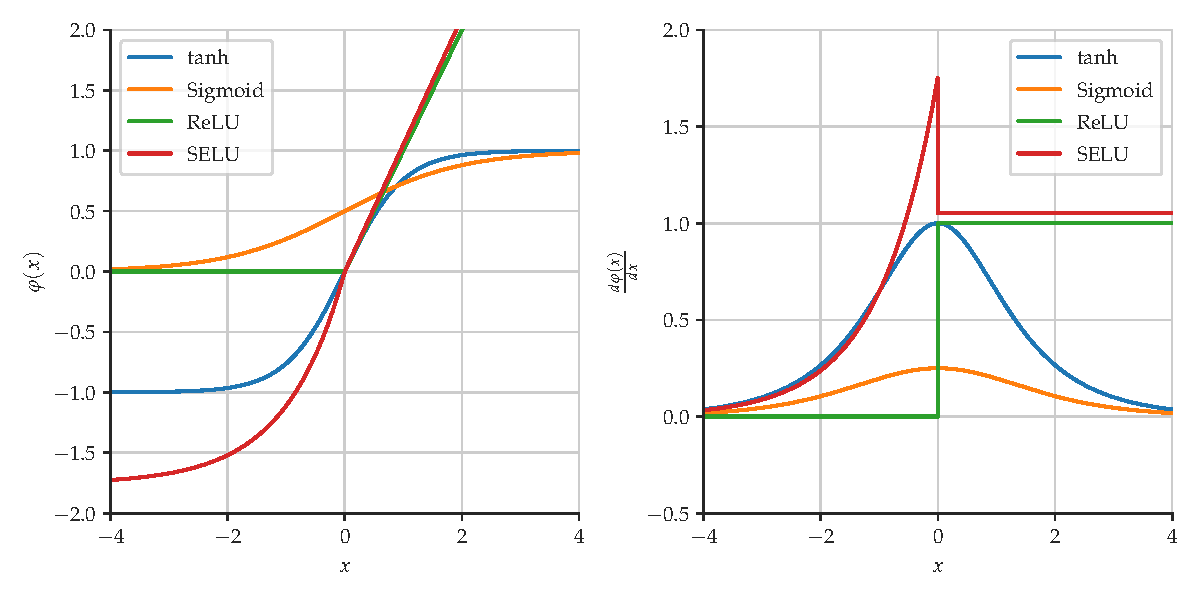
\includegraphics[scale = 0.7]{mlp-activations.pdf}
	\caption{À esquerda, algumas funções de ativação comuns em tarefas de predição e regressão para o neurônio \textit{Perceptron} e, à direita, suas derivadas}
	\label{fig:mlp-activations}
\end{figure}

É interessante mencionar o fato de que, assim como podemos selecionar uma gama de funções não-lineares para a ativação do neurônio, de forma a realizar transformações não-lineares na entrada, também é possível utilizar funções de ativação lineares, ou seja, realizar transformações lineares à semelhança dos modelos clássicos de predição. Nesse caso, a falta da não-linearidade tornaria muito difícil ou até mesmo impossibilitaria que sistemas mais complexos fossem descritos de forma aceitável por redes neurais artificiais desse tipo \cite{hornik1989multilayer}.

Tipicamente, uma rede neural MLP é composta por um número arbitrário $N_L$ de  camadas com $n$ neurônios do tipo \textit{Perceptron}, com a característica de que as saídas dos neurônios da $l$-ésima camada são propagadas para a frente, servindo como as entradas de todos os neurônios da camada seguinte ($l+1$). Esse processo é conhecido como \textit{feedforward}. Por isso, este tipo de rede é conhecida como totalmente conectada (ou densa) e pertence à categoria de modelos \textit{feedforward}. A Figura \ref{fig:mlp-architecture} apresenta a estrutura típica das redes MLP.

\begin{figure}[!ht]
\centering
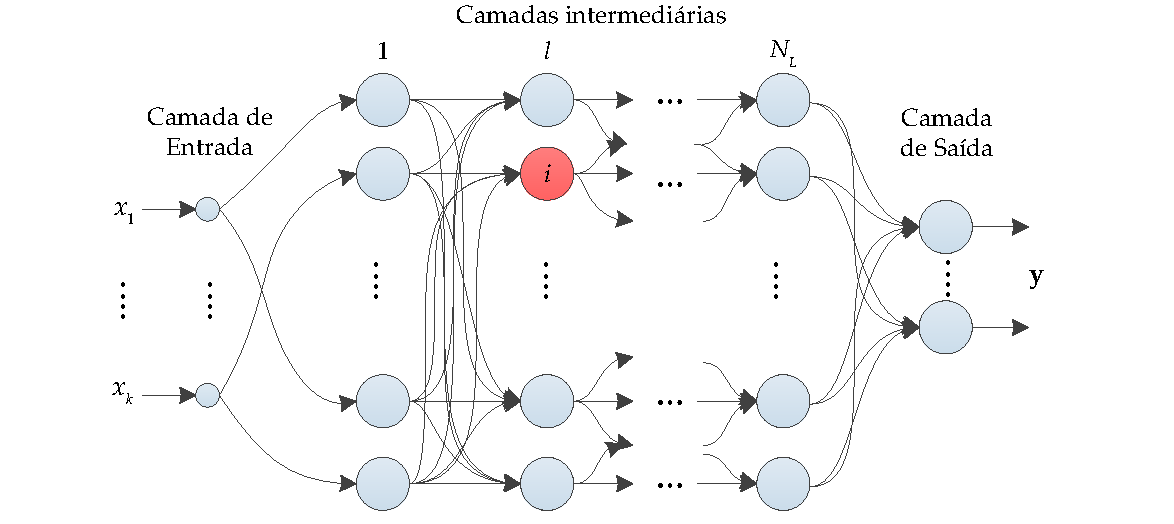
\includegraphics[scale = 0.8]{mlp-network.pdf}
\caption{Estrutura típica de uma rede MLP (figura adaptada de \cite{boccato2013novas}) }
\label{fig:mlp-architecture}
\end{figure}

Pela figura vemos que, além das $N_L$ camadas intermediárias com neurônios \textit{Perceptron}, a estrutura das redes MLP contém uma camada de entrada, que possui ativação linear e apenas passa o atributo de entrada relacionado ao neurônio específico ($x_1$, $x_2$, ..., $x_k$) para a primeira camada intermediária, e uma camada de saída que gera as respostas da rede neural para um vetor de entrada. A função de ativação da camada de saída e o número de neurônios presentes nela dependem da tarefa a ser realizada pela MLP. Por exemplo, em aplicações de regressão é comum o uso de um ou mais neurônios (dependendo se a saída do preditor será um vetor com um ou mais instantes de tempo) com função de ativação linear. Já em aplicações de classificação, a função de ativação pode variar entre a função logística (utilizada no caso binário em que queremos saber se uma entrada pertence ou não a uma classe) e a função \textit{softmax} (que gera uma saída para cada classe, indicando a probabilidade de uma entrada pertencer à classe em específico) e, novamente, o número de neurônios de saída também varia com o tipo da classificação.

Com base em (\ref{eq:mlp-out}), é possível representar a saída do $i$-ésimo neurônio da $l$-ésima camada intermediária da seguinte forma: 
\begin{equation}
	y_{i}^{l} = \varphi^{l} \Big(\sum_{j=1}^{n_{l-1}} w_{ij}^{l} y_{j}^{l-1} + w_{i0}^{l} \Big)\mathtt{,}
\end{equation}
onde $w_{ij}^{l}$ representa o peso sináptico da conexão que liga o $j$-ésimo neurônio da camada $l-1$ ao $i$-ésimo neurônio da camada $l$, sendo que na primeira camada intermediária os sinais de entrada são os atributos do vetor de entrada, ou seja, $y_{j}^{0} = x_{j}$ com $j = 1, ..., k$ \cite{boccato2013novas}. O parâmetro $n_{l-1}$ denota o número de neurônios na camada ($l-1$). 

O processo de treinamento de uma rede neural artificial normalmente é realizado com sequências de vetores de entrada $\mathbf{x}$, chamadas de \textit{mini-batch}, e chamamos um período de treinamento de época (do inglês \textit{epoch}) \cite{geron2019hands}. No treinamento, os pesos sinápticos $\mathbf{w}$ são ajustados em um processo iterativo de forma a minimizar uma função custo $J(\mathbf{w})$, a qual exprime uma medida do erro entre as saídas geradas pela rede e as saídas desejadas (vale mencionar que $\mathbf{w}$ é um vetor com todos os parâmetros da rede). No caso de um problema de regressão ou predição, é comum que a função custo a ser minimizada seja o Erro Quadrático Médio (MSE, do inglês \textit{Mean Squared Error}). De qualquer forma, o treinamento de uma rede neural dá origem a um problema de otimização não-linear irrestrita \cite{haykin2010neural}.

Para isso, é frequente o uso de algoritmos de otimização baseados em derivadas da função custo $J(\mathbf{w})$, como o método do gradiente descendente estocástico (SGD, do inglês \textit{stochastic gradient descent}), o método de Nesterov (NAG, do inglês \textit{Nesterov Accelerated Gradient}) e o algoritmo Adam (\textit{Adaptive Moment Estimation}) \cite{geron2019hands}. O famoso algoritmo de retropropagação (\textit{backpropagation}) do erro, cuja representação matemática também varia de acordo com o tipo de otimização, é empregado para viabilizar o cálculo das derivadas com relação aos pesos sinápticos dos neurônios situados nas camadas internas da rede, de forma que, para cada \textit{mini-batch}, seja possível atualizar todos os pesos de todos os neurônios presentes em todas as camadas. 

Nesse caso, é comum dividirmos os métodos de otimização entre métodos de primeira ordem e de segunda ordem. Os métodos de primeira ordem utilizam as derivadas de primeira ordem da função custo, geralmente representadas com o uso do vetor gradiente:
\begin{equation}
	\nabla J(\mathbf{w}) = \Big[\frac{\partial J(\mathbf{w})}{\partial w_1} \; ...\;  \frac{\partial J(\mathbf{w})}{\partial w_n} \Big]^T
\end{equation}

Assim, ao caminharmos na direção contrária à apontada pelo vetor $\nabla J(\mathbf{w})$ obtemos, de forma iterativa, a minimização desejada. Logo, a regra de atualização dos pesos pode ser dada pela forma básica:
\begin{equation}\label{mlp-w-basic}
	\mathbf{w}[k+1] \leftarrow \mathbf{w}[k] - \eta \nabla J \big[\mathbf{w}[k]\big]
\end{equation} 

Os algoritmos de otimização mencionados (SGD, Adam, NAG) utilizam variações da regra de atualização de $\mathbf{w}$ indicada em (\ref{mlp-w-basic}).

Para esta pesquisa, optamos por utilizar o algoritmo Nadam (\textit{Nesterov Adaptive Moment Estimation}) \cite{dozat2016incorporating}. O Nadam, como o nome já sugere, incorpora elementos dos algoritmos NAG e Adam, de forma a ter um passo de atualização adaptativo e com acúmulo dos gradientes mais recentes (semelhante à ideia de momento linear de uma partícula), com a utilização do "truque de Nesterov", desenvolvido pelo matemático russo Yurii Nesterov \cite{nesterov1983method}, onde o gradiente não é calculado sobre o ponto atual indicado pelo vetor $\mathbf{w}$, mas sim sobre um ponto levemente à frente, na mesma direção do momento. O conjunto de equações que descreve o algoritmo Nadam é dado por:
\begin{subequations}
\begin{equation}\label{eq:nadam-1}
 \mathbf{w}' = \mathbf{w} + \beta_{3} \mathbf{m}
\end{equation}
\begin{equation}\label{eq:nadam-2}
 \mathbf{m} \leftarrow \beta_{1}\mathbf{m} - (1 - \beta_{1}) \nabla_{\mathbf{w}}E(\mathbf{w}')
\end{equation}
\begin{equation}\label{eq:nadam-3}
 \mathbf{s} \leftarrow \beta_{2}\mathbf{s} - (1 - \beta_{2}) \nabla_{\mathbf{w}}E(\mathbf{w}') \otimes \nabla_{\mathbf{w}}E(\mathbf{w}') 
\end{equation}
\begin{equation}\label{eq:nadam-4}
\hat{\mathbf{m}} \leftarrow \frac{\mathbf{m}}{1 - \beta_{1}}
\end{equation}
\begin{equation}\label{eq:nadam-5}
\hat{\mathbf{s}} \leftarrow \frac{\mathbf{s}}{1 - \beta_{2}}
\end{equation}
\begin{equation}\label{eq:nadam-6}
 \mathbf{w} \leftarrow \mathbf{w} + \eta \hat{\mathbf{m}} \oslash \sqrt{\hat{\mathbf{s}} + \epsilon}
\end{equation}
\end{subequations}

A incorporação dos gradientes passados no cálculo do próximo vetor $\mathbf{w}$ ocorre através da equação (\ref{eq:nadam-2}), que define o vetor de momento $\mathbf{m}$. Assim, utilizando a analogia com o momento linear de uma partícula, o gradiente passa ter a ideia de uma força de aceleração que aumenta o valor do momento do vetor $\mathbf{w}$ caso este esteja indo para um ponto ótimo de mínimo local, escapando mais rapidamente de regiões onde não há minimização significativa da função custo.

O hiperparâmetro $\beta_1$ presente em (\ref{eq:nadam-2}) serve tanto para evitar que $\mathbf{m}$ aumente de forma descontrolada, como também para fazer com que, através do termo $(1 - \beta_1)$, surja uma média exponencialmente decrescente de valores anteriores. Normalmente, $\beta_1$ é inicializado em $0.9$.

Já o vetor $\mathbf{s}$, definido em (\ref{eq:nadam-3}), serve para evitar que o algoritmo de otimização caminhe com uma direção que não aponte para o ponto ótimo mencionado anteriormente. Além disso, para evitar que esse ajuste na direção cause uma perda significativa na rapidez de convergência do algoritmo, utiliza-se os termos $\beta_2$ e $(1 - \beta_2)$, ou seja, um decaimento exponencial nos valores passados de $\mathbf{s}$. Nesse caso, o hiperparâmetro $\beta_2$ é inicializado em $0.999$ e $\epsilon$ em $10^{-7}$ (para evitar uma divisão por zero).

Por fim, as equações (\ref{eq:nadam-4}) e (\ref{eq:nadam-5}) servem para corrigir um possível viés dos vetores $\mathbf{m}$ e $\mathbf{s}$ devido à estratégia típica de inicialização (a saber, para valores próximos a $0$). 

É importante mencionar que os métodos de otimização aqui mencionados são métodos de busca local, ou seja, têm convergência esperada para um mínimo local, que não necessariamente é o mínimo global da função custo para a aplicação. Dizemos também que esses pontos mínimos possuem "bacias de atração" que, para valores adequados da taxa de aprendizado $\eta$, atraem o vetor de parâmetros $\mathbf{w}$ \cite{hastie2009elements}.

Um fenômeno possivelmente presente durante o treinamento da rede neural é o desaparecimento dos gradientes (do inglês \textit{vanishing gradients problem}) nas camadas inferiores da rede, ou o aumento desenfreado desses gradientes (do inglês \textit{exploding gradients problem}) nas camadas citadas, que é mais comum para redes recorrentes. Para evitar que isso ocorra, normalmente são utilizadas camadas que realizam uma normalização do \textit{batch} de vetores de entrada (BN, do inglês \textit{Batch Normalization}), sendo posicionadas antes ou depois das camadas intermediárias da rede \cite{geron2019hands}.

De forma resumida, o que a BN faz é remover a média e padronizar os desvios de todas as variáveis em sua presente, conforme a informação disponível no \textit{mini-batch} atual, para, depois, redefinir tais medidas com parâmetros que devem ser determinados pelo treinamento. Ou seja, a camada BN tenta identificar a forma de melhor remodelar as variáveis de entrada em termos de suas médias e desvios padrão. A transformação aplicada pela BN pode ser representada pelas seguintes equações: 
\begin{subequations}
\begin{equation}\label{eq:bn-1}
 \boldsymbol{\mu}_{B} = \frac{1}{d} \sum_{i=1}^{d} \mathbf{x}_{i} 
\end{equation}
\begin{equation}\label{eq:bn-2}
\boldsymbol{\sigma}_{B}^{2} = \frac{1}{d} \sum_{i=1}^{d} (\mathbf{x}_{i} - \boldsymbol{\mu}_{B})^2 
\end{equation}
\begin{equation}\label{eq:bn-3}
\hat{\mathbf{x}}_{i} = \frac{\mathbf{x}_{i} - \boldsymbol{\mu}_{B}}{\sqrt{\boldsymbol{\sigma}_{B}^2 + \epsilon}}
\end{equation}
\begin{equation}\label{eq:bn-4}
\mathbf{z}_{i} = \boldsymbol{\gamma} \otimes \hat{\mathbf{x}}_{i} + \boldsymbol{\beta}
\end{equation}
\end{subequations}
sendo $\boldsymbol{\mu}_{B}$ e $\boldsymbol{\sigma}_{B}$ os vetores com as médias e desvios-padrão para cada atributo de entrada do atual \textit{mini-batch} (este contendo $d$ vetores $\mathbf{x}$), $\hat{\mathbf{x}}_{i}$ é o $i$-ésimo vetor de entrada centrado em zero e normalizado, $\boldsymbol{\gamma}$ é o vetor que pondera cada um dos atributos de $\hat{\mathbf{x}}_{i}$, $\boldsymbol{\beta}$ tem um termo de \textit{offset} para cada atributo normalizado, $\epsilon$ novamente é um termo pequeno (geralmente na ordem de $10^{-5}$) para evitar uma divisão por zero e, por fim, $\mathbf{z}_{i}$ é a saída da camada de \textit{batch normalization}.

Os hiperparâmetros $\boldsymbol{\beta}$ e $\boldsymbol{\gamma}$ controlam o deslocamento e o escalonamento, respectivamente, de cada atributo para um vetor de entrada. Essas variáveis são parametrizadas durante o treinamento da rede neural de forma bem eficiente dependendo da quantidade e do tamanho dos \textit{mini-batches}. 

Também vale mencionar que, para o conjunto de dados de validação, ou seja, o conjunto de dados que, após o ajuste dos pesos $\mathbf{w}$ no conjunto de treinamento, é verificado se a rede neural está generalizando os resultados, evitando o sobreajuste (do inglês \textit{overfitting}), são calculados outros vetores de valores de média ($\boldsymbol{\mu}_{B}'$) e desvios-padrão ($\boldsymbol{\sigma}_{B}'$), a partir de médias móveis com decaimento exponencial. Assim, o processo descrito anteriormente também é realizado sobre esses dados.

Por fim, o grande apelo das redes \textit{Multilayer Perceptron} é que elas possuem capacidade de aproximação universal, ou seja, são capazes de aproximar qualquer mapeamento contínuo num domínio compacto com um nível de erro arbitrariamente pequeno. Até mesmo uma MLP com uma única camada intermediária e camada de saída linear já possui esta capacidade \cite{cybenko1989approximation, hornik1989multilayer}. Infelizmente, esse teorema não indica a quantidade de neurônios necessária na(s) camada(s) intermediária(s), muito menos um método para ajustar o vetor $\mathbf{w}$ da rede para garantir a solução ótima.

Além disso, para o propósito deste trabalho de pesquisa, que envolve sistemas dinâmicos, ter acesso a um histórico e a uma memorização dos padrões anteriores de entrada, na teoria, aumentaria a precisão da predição das séries temporais. Mesmo que as redes MLP tenham capacidade de aproximação universal, é possível aumentar a flexibilidade desse processo caso fossem utilizadas estruturas recorrentes \cite{connor1994recurrent, boccato2013novas}.

Logo, incluímos na análise alguns modelos de redes neurais recorrentes. Discutiremos mais sobre a estrutura e o funcionamento delas na próxima seção.

\subsubsection{Redes Neurais Recorrentes (RNN)} 
Diferentemente das redes MLP que são \textit{feedforward}, ou seja, que não reutilizam a informação processada dos padrões anteriores para gerar a próxima saída, a ideia central das redes neurais recorrentes (RNN, do inglês \textit{Recurrent Neural Networks}) é que elas têm estruturas computacionais que podem armazenar os estados anteriores dos neurônios, podendo também possuir portas não-lineares que regulam o fluxo de informação de entrada e de saída da célula computacional \cite{haykin2010neural}. Uma representação possível de uma célula básica de uma rede recorrente pode ser vista na Figura \ref{fig:recorrente-cell} (esquerda).
\begin{figure}[H]
\centering
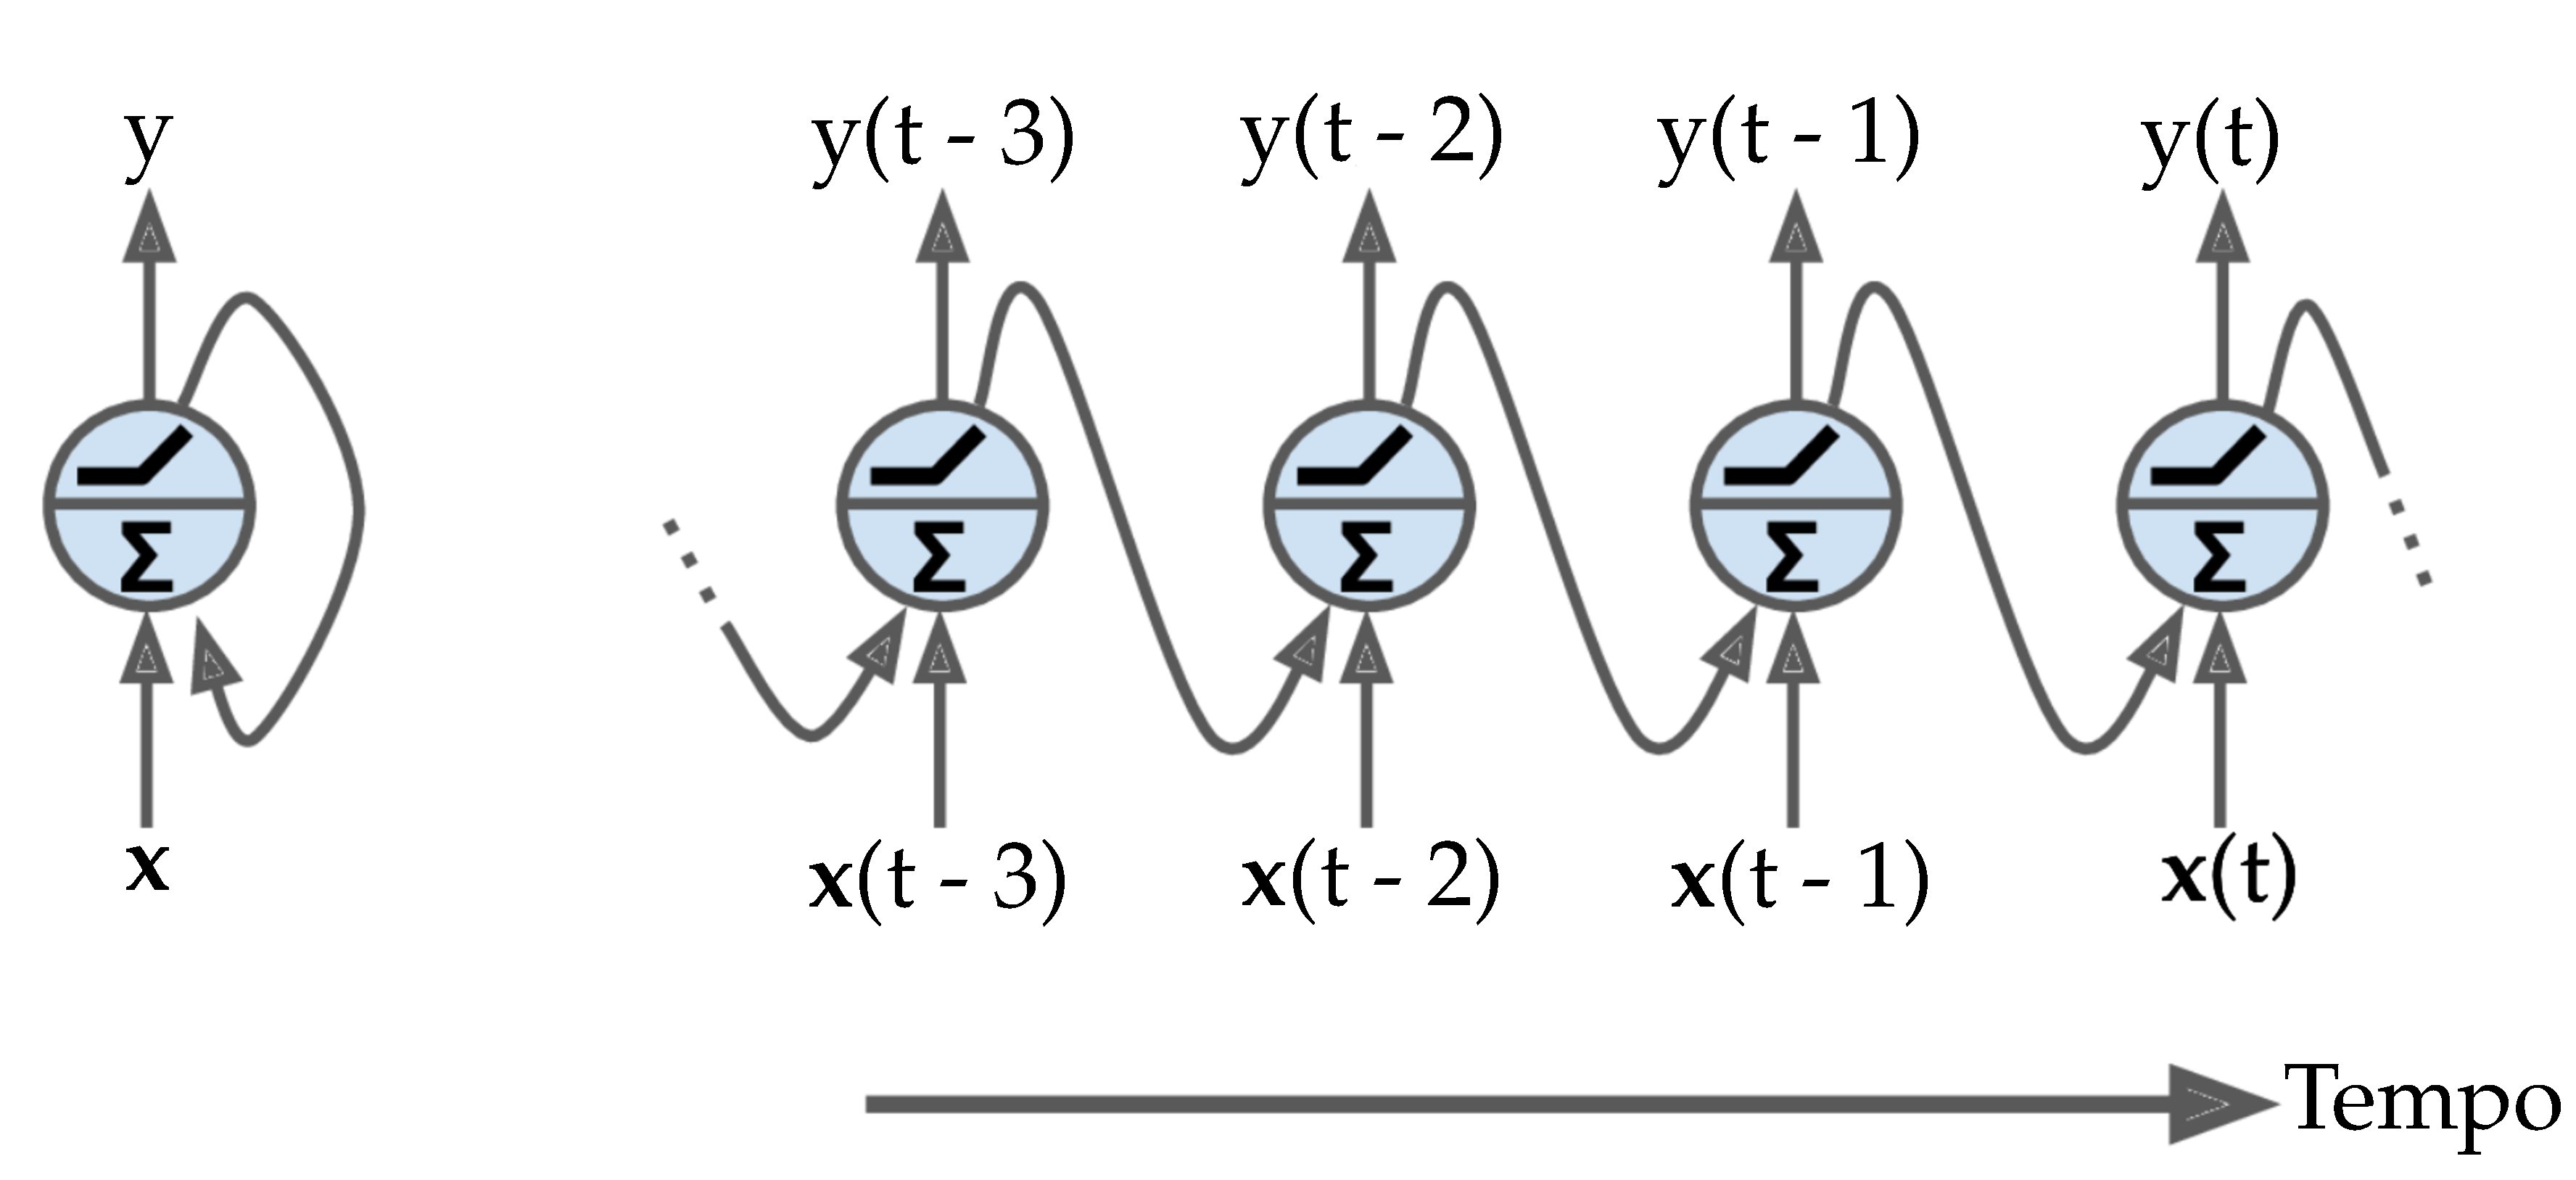
\includegraphics[scale = 0.2]{rnn-cell.pdf}
\caption{À esquerda, célula básica da rede recorrente e, à direita, sua representação através do tempo (figura adaptada de \cite{geron2019hands})}
\label{fig:recorrente-cell}
\end{figure}

Note que a saída é realimentada (com um atraso temporal) para a entrada do próprio neurônio. Assim, a célula recorrente recebe tanto o vetor de entradas $\mathbf{x}(t)$ assim como a saída no instante anterior $y(t-1)$ que, devido à relação de recorrência, reflete implicitamente as saídas em todos os instantes anteriores $y(t-k)$ com $1 < k \leq t$ (considerando $y(0)$). Dessa forma, como pode ser visto na Figura \ref{fig:recorrente-cell} (direita), é possível representar essa rede ao longo do tempo, através de um processo chamado desenrolamento da rede no tempo (do inglês \textit{unrolling the network through time}) \cite{geron2019hands}.

Uma camada recorrente é formada de maneira similar à célula, com a diferença que cada neurônio recebe, além do vetor de entradas $\mathbf{x}(t)$, um vetor de saídas $\mathbf{y}(t-1)$, que contém as saídas de todos as unidades recorrentes da camada em instantes anteriores, conforme a Figura \ref{fig:recorrente-camada} indica. 
\begin{figure}[H]
\centering
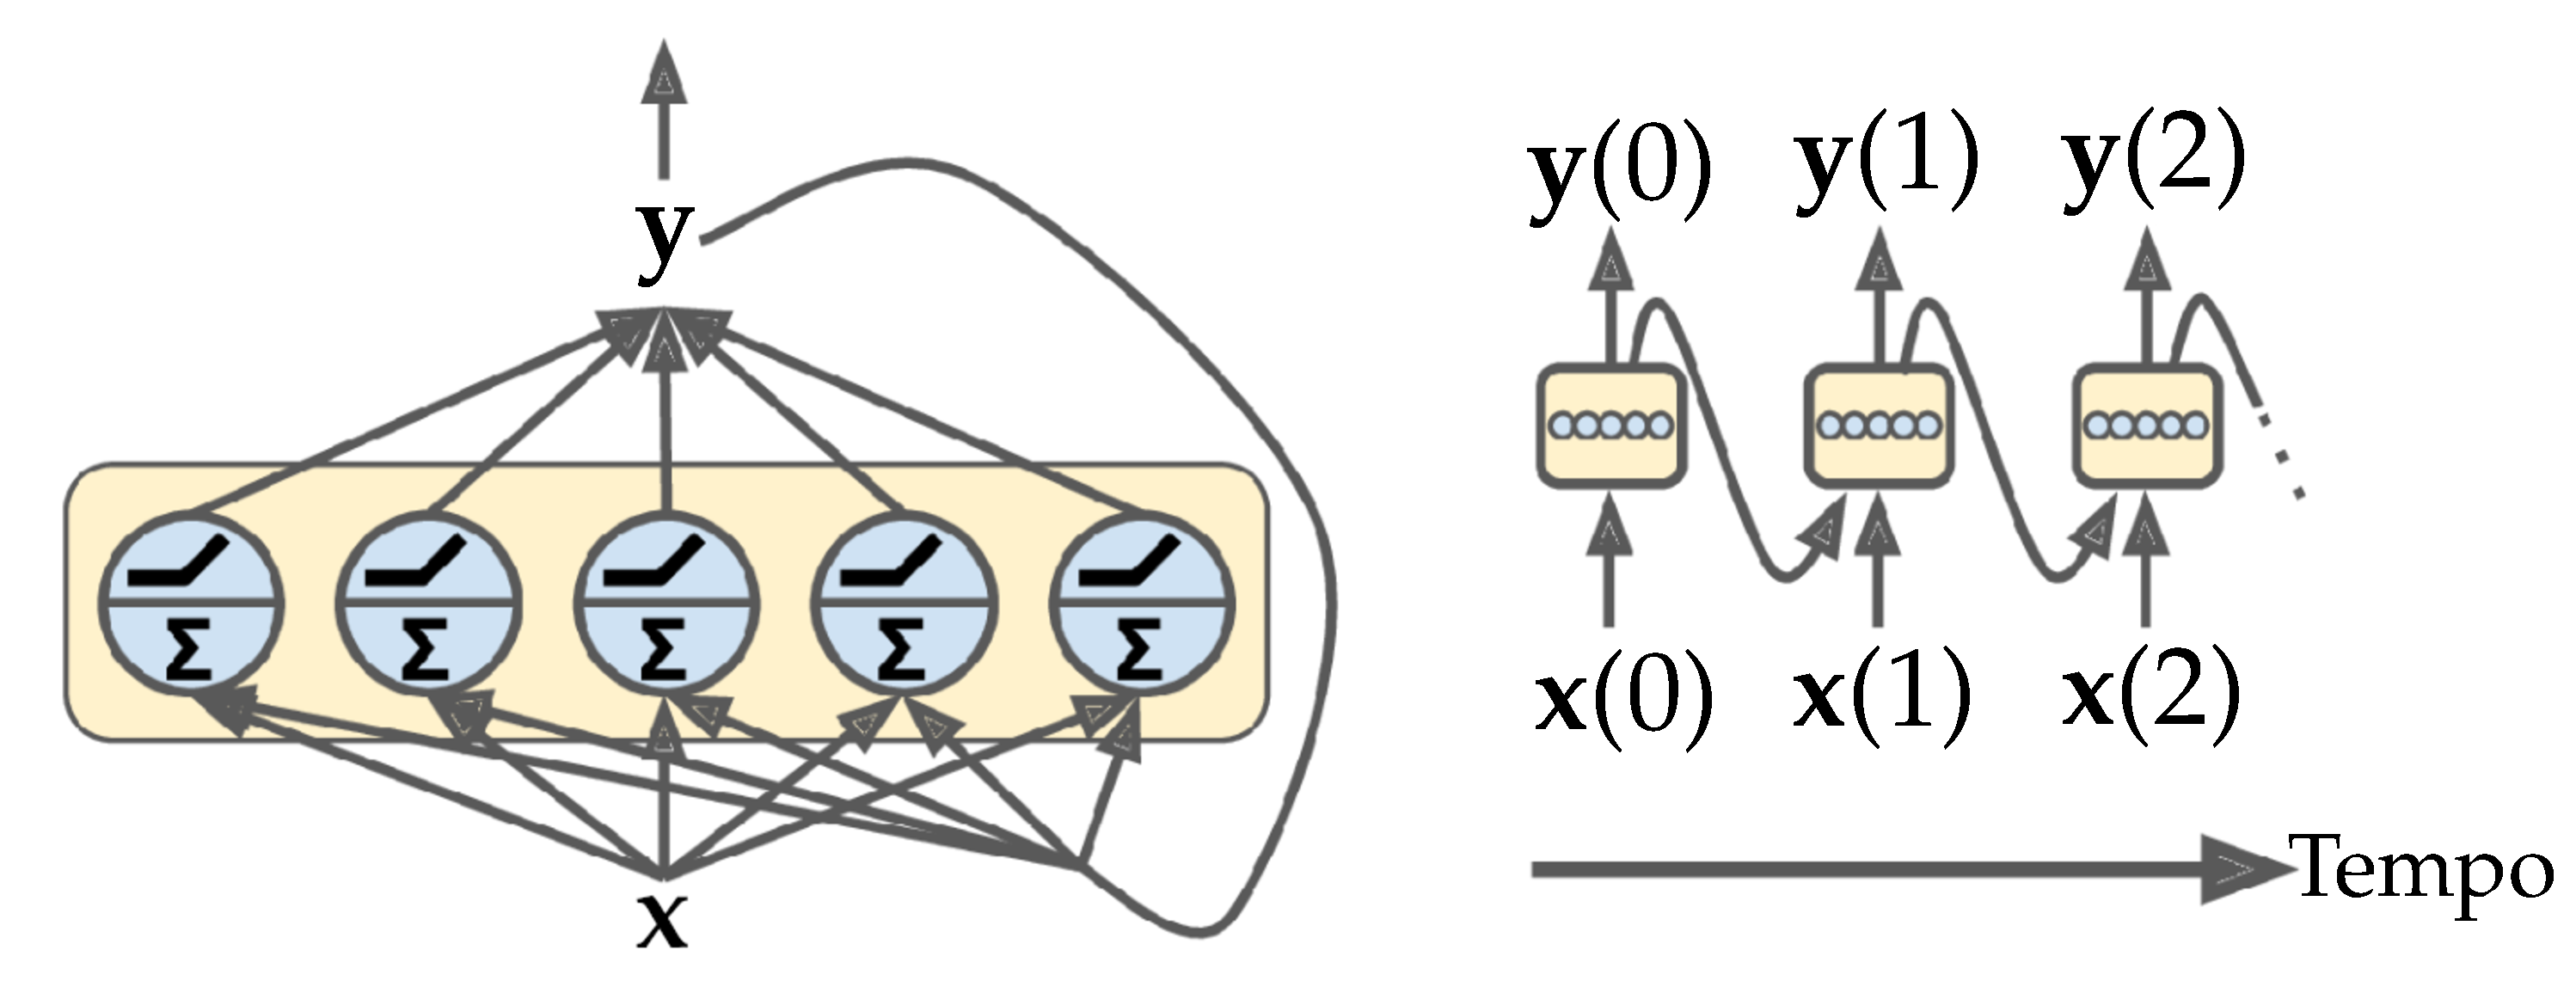
\includegraphics[scale = 0.25]{rnn-layer.pdf}
\caption{À esquerda, camada da rede recorrente e, à direita, sua representação através do tempo (figura adaptada de \cite{geron2019hands})}
\label{fig:recorrente-camada}
\end{figure}

Dessa forma, cada célula recorrente possui dois vetores de pesos, $\mathbf{w}_x$ e $\mathbf{w}_y$. O primeiro pondera o vetor de entradas $\mathbf{x}(t)$, de forma similar à apresentada anteriormente na MLP, enquanto o vetor $\mathbf{w}_y$ pondera o vetor das saídas dos estados passados $\mathbf{y}(t-1)$.

Logo, pode-se formar uma camada recorrente agrupando os vetores de pesos de cada célula nas matrizes $\mathbf{W}_x$ e $\mathbf{W}_y$, sendo que a saída da camada, isto é, $\mathbf{y}(t)$, é dada por:
\begin{equation}\label{eq:rnn-layer}
\mathbf{y}(t) = \varphi \big(\mathbf{W}_x \mathbf{x}(t) + \mathbf{W}_y \mathbf{y}(t-1) + \mathbf{b} \big)
\end{equation}

Assim, devido à presença do vetor $\mathbf{y}(t-1)$ em (\ref{eq:rnn-layer}), a saída da camada recorrente no instante $t$ acaba sendo influenciada por todas as entradas anteriores ($\mathbf{x}(0)$, $\mathbf{x}(1)$, ... $\mathbf{x}(t-1)$). Devido a isso, é dito que a rede recorrente possui uma memória dos estados anteriores \cite{geron2019hands}. 

Em geral, o estado atual de uma célula é representado através de uma função $\mathbf{h}(t)$, de forma a termos a seguinte relação entre $\mathbf{h}(t)$ e $\mathbf{y}(t)$:
\begin{equation}
	\mathbf{h}(t) = f(\mathbf{x}(t), \mathbf{h}(t-1))
\end{equation}
\begin{equation}
	\mathbf{y}(t) = g(\mathbf{x}(t), \mathbf{h}(t-1))
\end{equation}

Nas células mais básicas apresentadas anteriormente, temos que $f(\mathbf{x}(t), \mathbf{h}(t-1)) = g(\mathbf{x}(t), \mathbf{h}(t-1))$, mas esse nem sempre é o caso. Assim, uma representação mais geral de uma célula recorrente pode ser vista na Figura \ref{fig:recorrente-cell-geral}.
\begin{figure}[!ht]
\centering
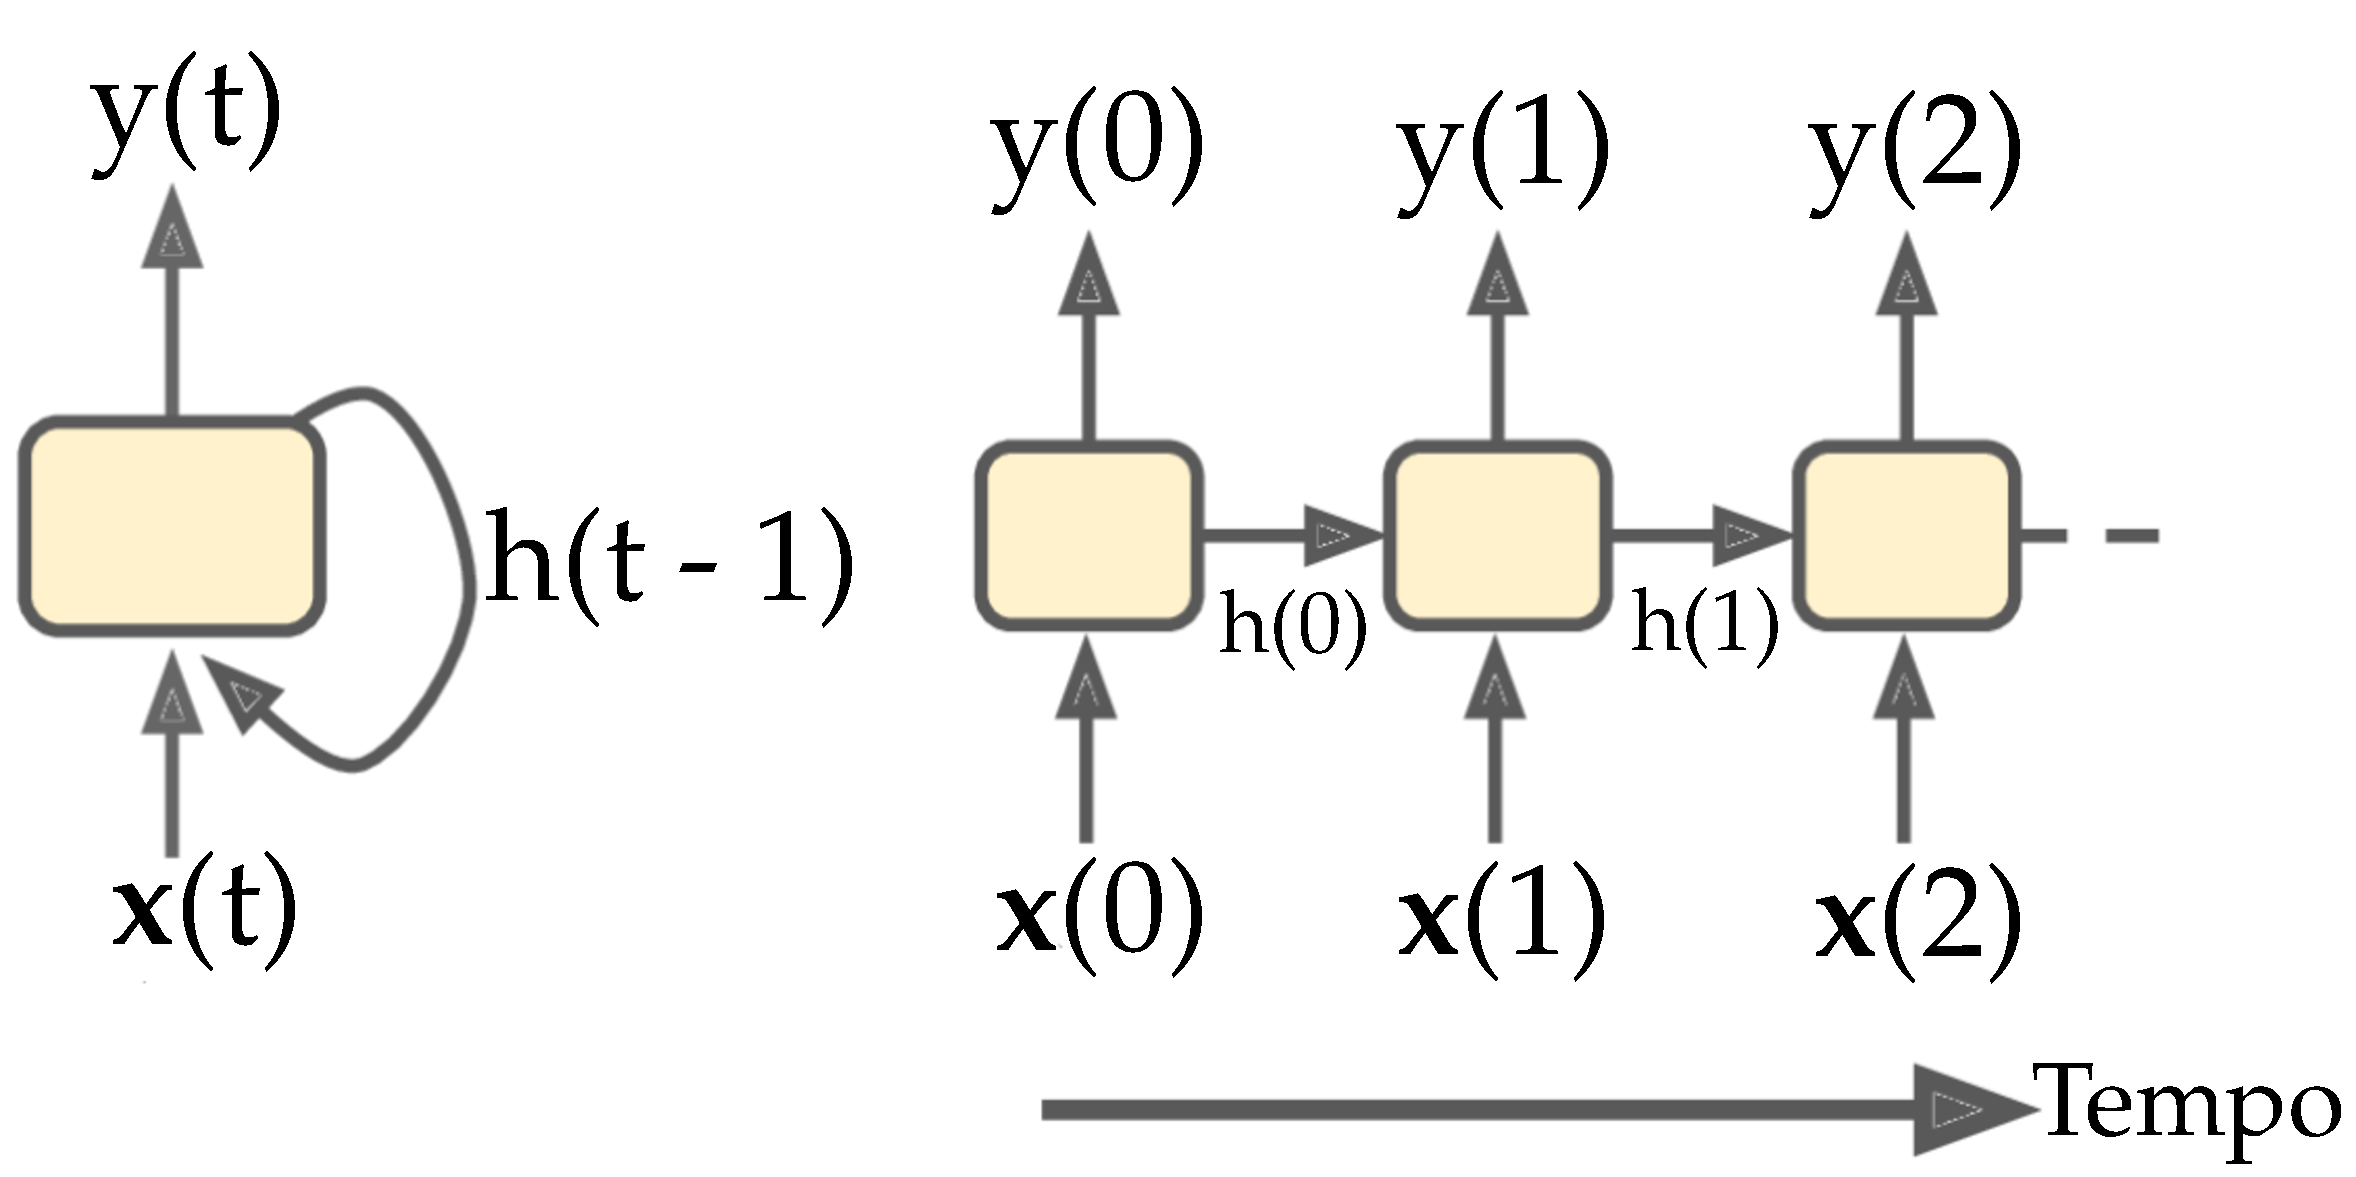
\includegraphics[scale = 0.25]{rnn-cell-general.pdf}
\caption{À esquerda, representação geral da célula da rede recorrente e, à direita, sua representação através do tempo (figura adaptada de \cite{geron2019hands})}
\label{fig:recorrente-cell-geral}
\end{figure}

A saída de uma RNN varia com a aplicação. Para a predição de séries temporais, utilizamos o arranjo sequência para sequência (do inglês \textit{sequence-to-sequence network}). Neste caso, a rede recebe uma sequência de entradas e gera uma sequência de saídas. Por exemplo, sendo $x(t)$ o valor da série temporal, $y(t)$ é a estimação da rede para o instante $t + L$, sendo $L$ o passo de predição. Logo, fornecendo em $t=0$ vetores de entrada um a um, as saídas serão as estimações dos valores para os instantes $1$ a $N + L$, sendo $N$ o número de amostras da série. 

Outro tipo de configuração possível para a predição de séries temporais é o arranjo sequência para vetor (do inglês \textit{sequence-to-vector network}), onde ignoramos todas as saídas com exceção da última. Assim, com esse arranjo é possível predizer os próximos $L$ valores desconhecidos da série. Essa configuração também é muito utilizada para gerar, com base em uma frase, um \textit{score} para o sentimento que foi transmitido pelo autor \cite{geron2019hands}.

Além disso, também é possível termos um arranjo vetor para sequência (do inglês \textit{vector-to-sequence network}). Esse tipo não é tanto utilizada para a predição de séries temporais, sendo mais utilizada para gerar legendas para imagens. 

Por fim, podemos combinar o esquema sequência-vetor seguido do vetor-sequência. Essa configuração é chamada de \textit{Encoder-Decoder}, utilizado para gerar traduções com base em uma frase. O \textit{Encoder} recebe uma sequência de palavras como entrada, gerando um vetor que é decodificado pelo \textit{Decoder} para formar o texto em outro idioma. A Figura \ref{fig:rnn-output-style} exibe as configurações possíveis.
\begin{figure}[!ht]
\centering
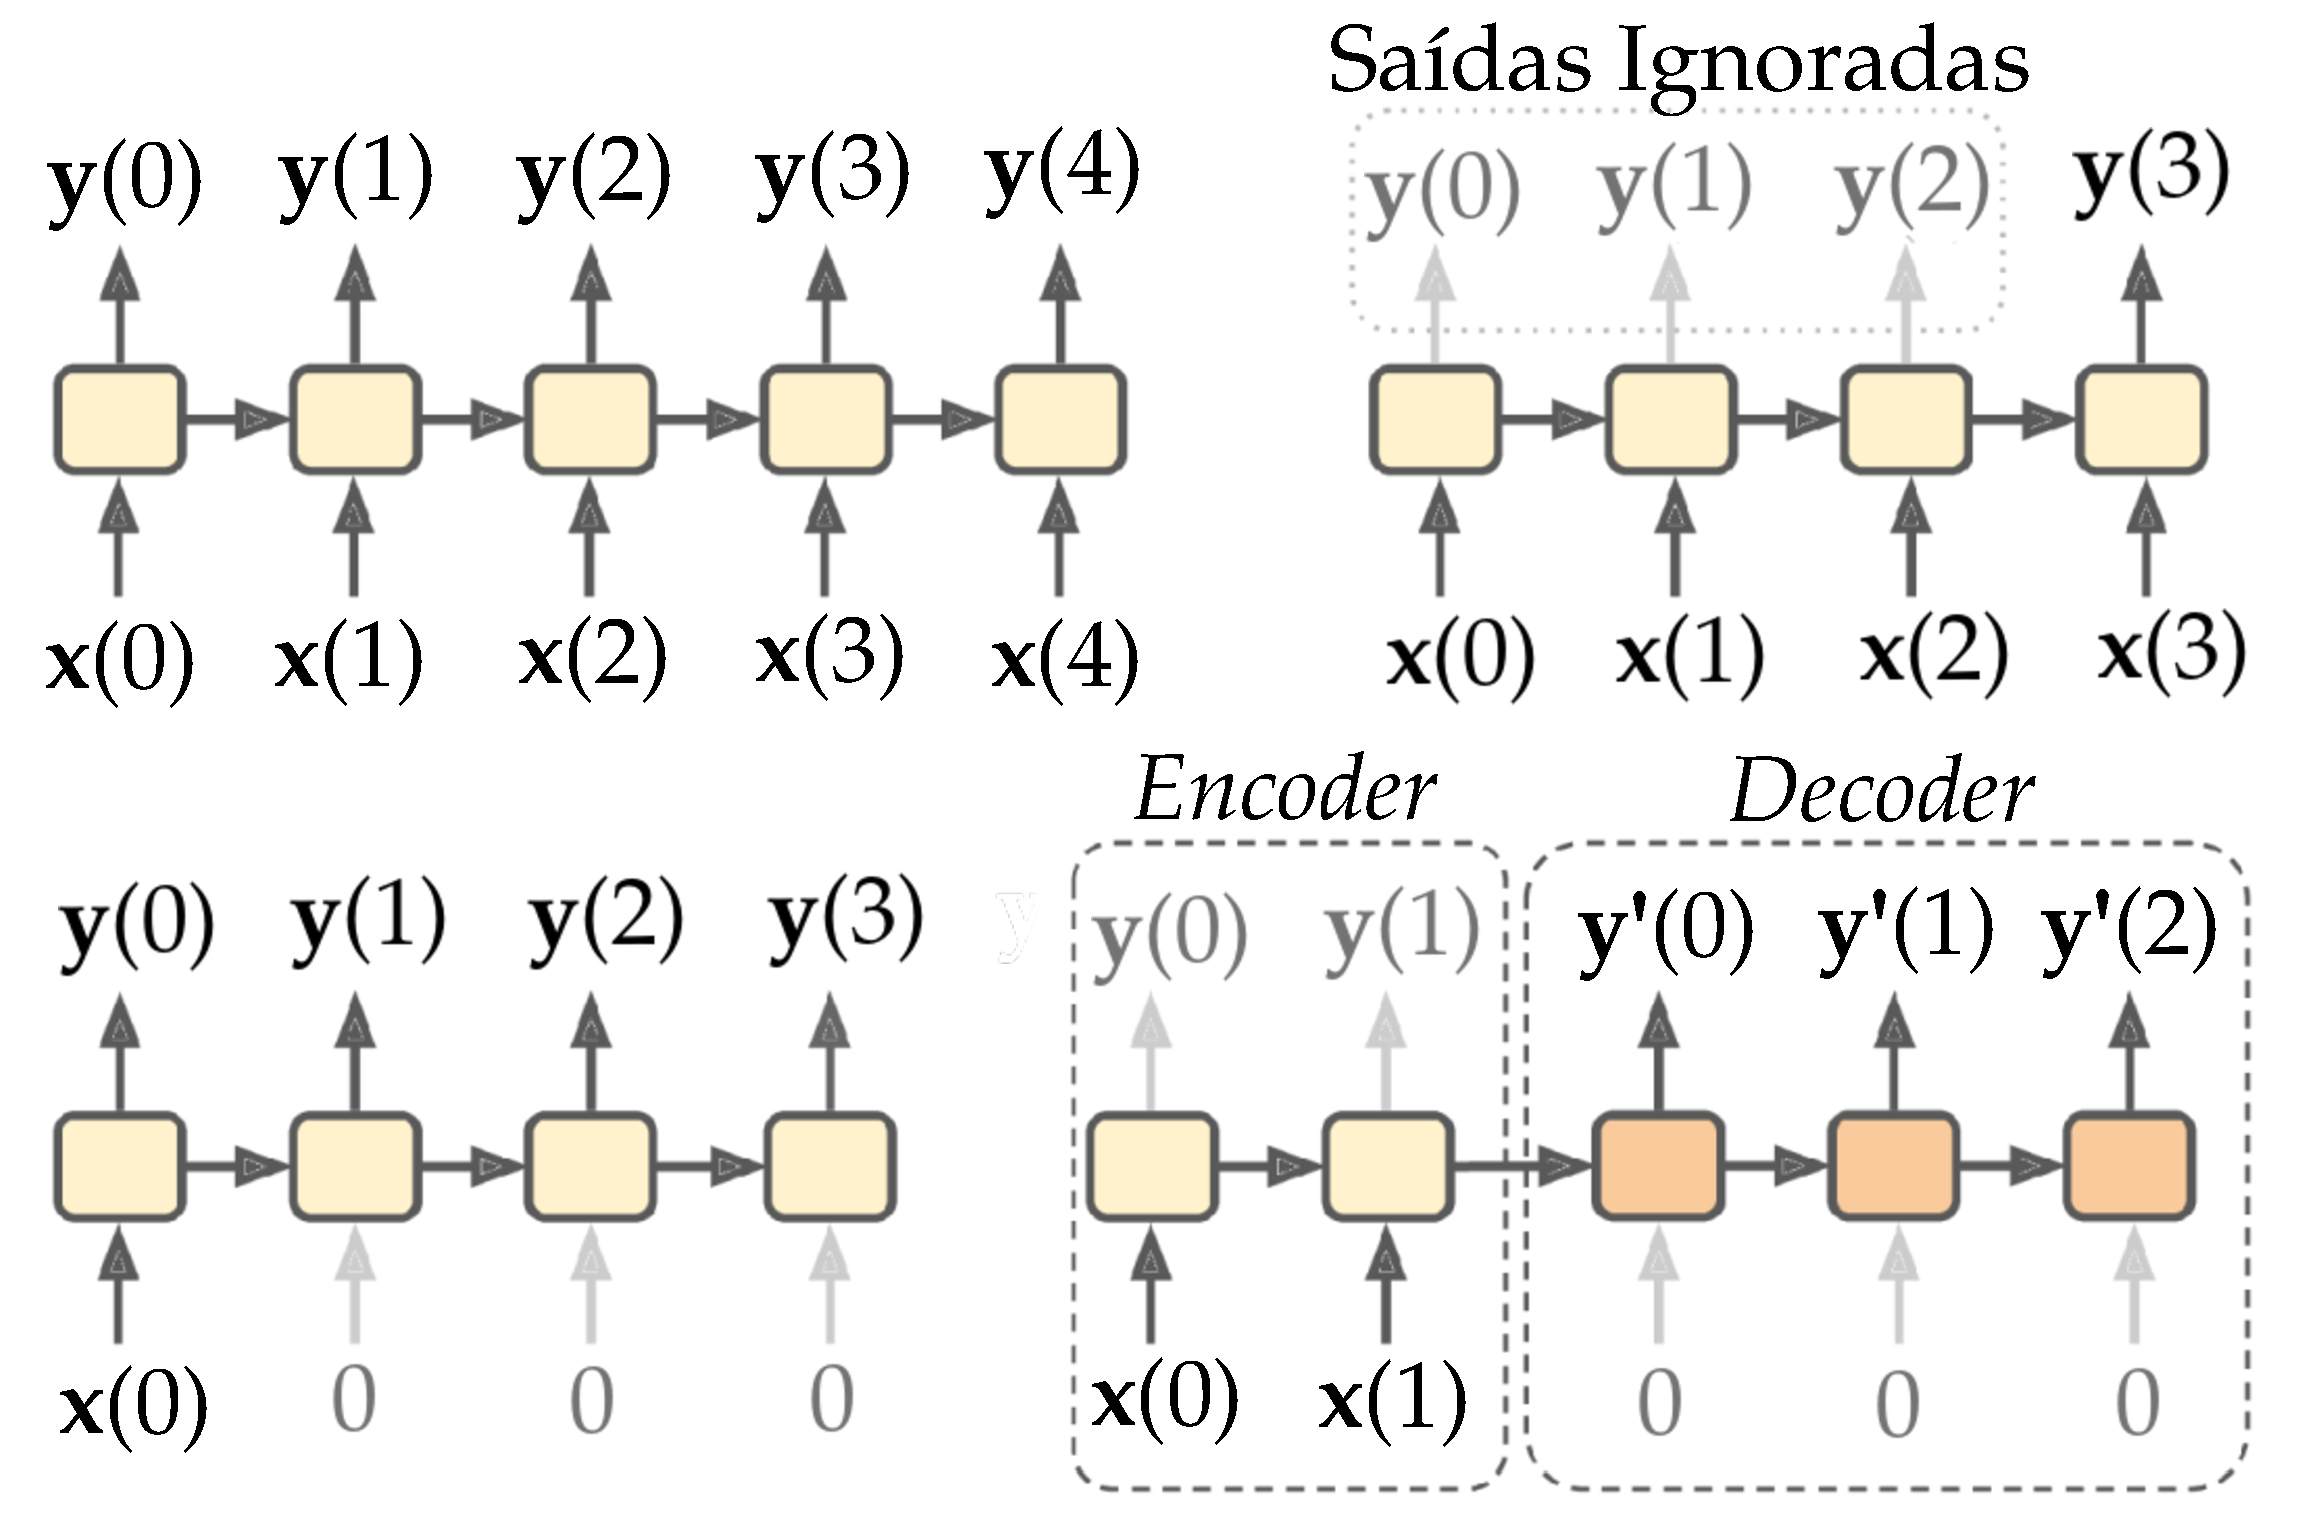
\includegraphics[scale = 0.3]{rnn-output-style.pdf}
\caption{Maneiras de se implementar uma RNN (figura adaptada de \cite{geron2019hands})}
\label{fig:rnn-output-style}
\end{figure}

O treinamento de uma rede recorrente também utiliza a técnica de retropropagação do erro, citada anteriormente quando foi discutida a rede MLP. A diferença é que o erro também deve ser retropropagado para $k$ instantes anteriores de tempo. Esta extensão da técnica é chamada de retropropagação do erro através do tempo (BPTT, do inglês \textit{backpropagation through time}).

Para compreender os pontos principais do funcionamento desse algoritmo, convém considerar a rede desdobrada no tempo (Figura \ref{fig:recorrente-camada}). Dessa forma, pode-se perceber que uma rede recorrente desdobrada no tempo é bem semelhante a uma rede \textit{feedforward} profunda, em que as várias camadas que representam a rede em instantes de tempo diferente compartilham os mesmos parâmetros.

Nesse caso, a entrada de camada da rede desdobrada corresponde ao vetor de entrada para um determinado instante de tempo. Logo, a camada correspondente ao primeiro instante de tempo recebe a entrada $\mathbf{x}(t-k)$, a camada seguinte a ela recebe a entrada $\mathbf{x}(t-k+1)$, e isso ocorre até a camada mais recente no tempo da rede, que recebe a entrada $\mathbf{x}(t)$. Também é válido mencionar que as saídas de determinados instantes de tempo podem ser ignoradas ao calcular a função custo $J$ para a rede desdobrada, assim como indica a Figura \ref{fig:rnn-backpropagation}.
\begin{figure}[!ht]
\centering
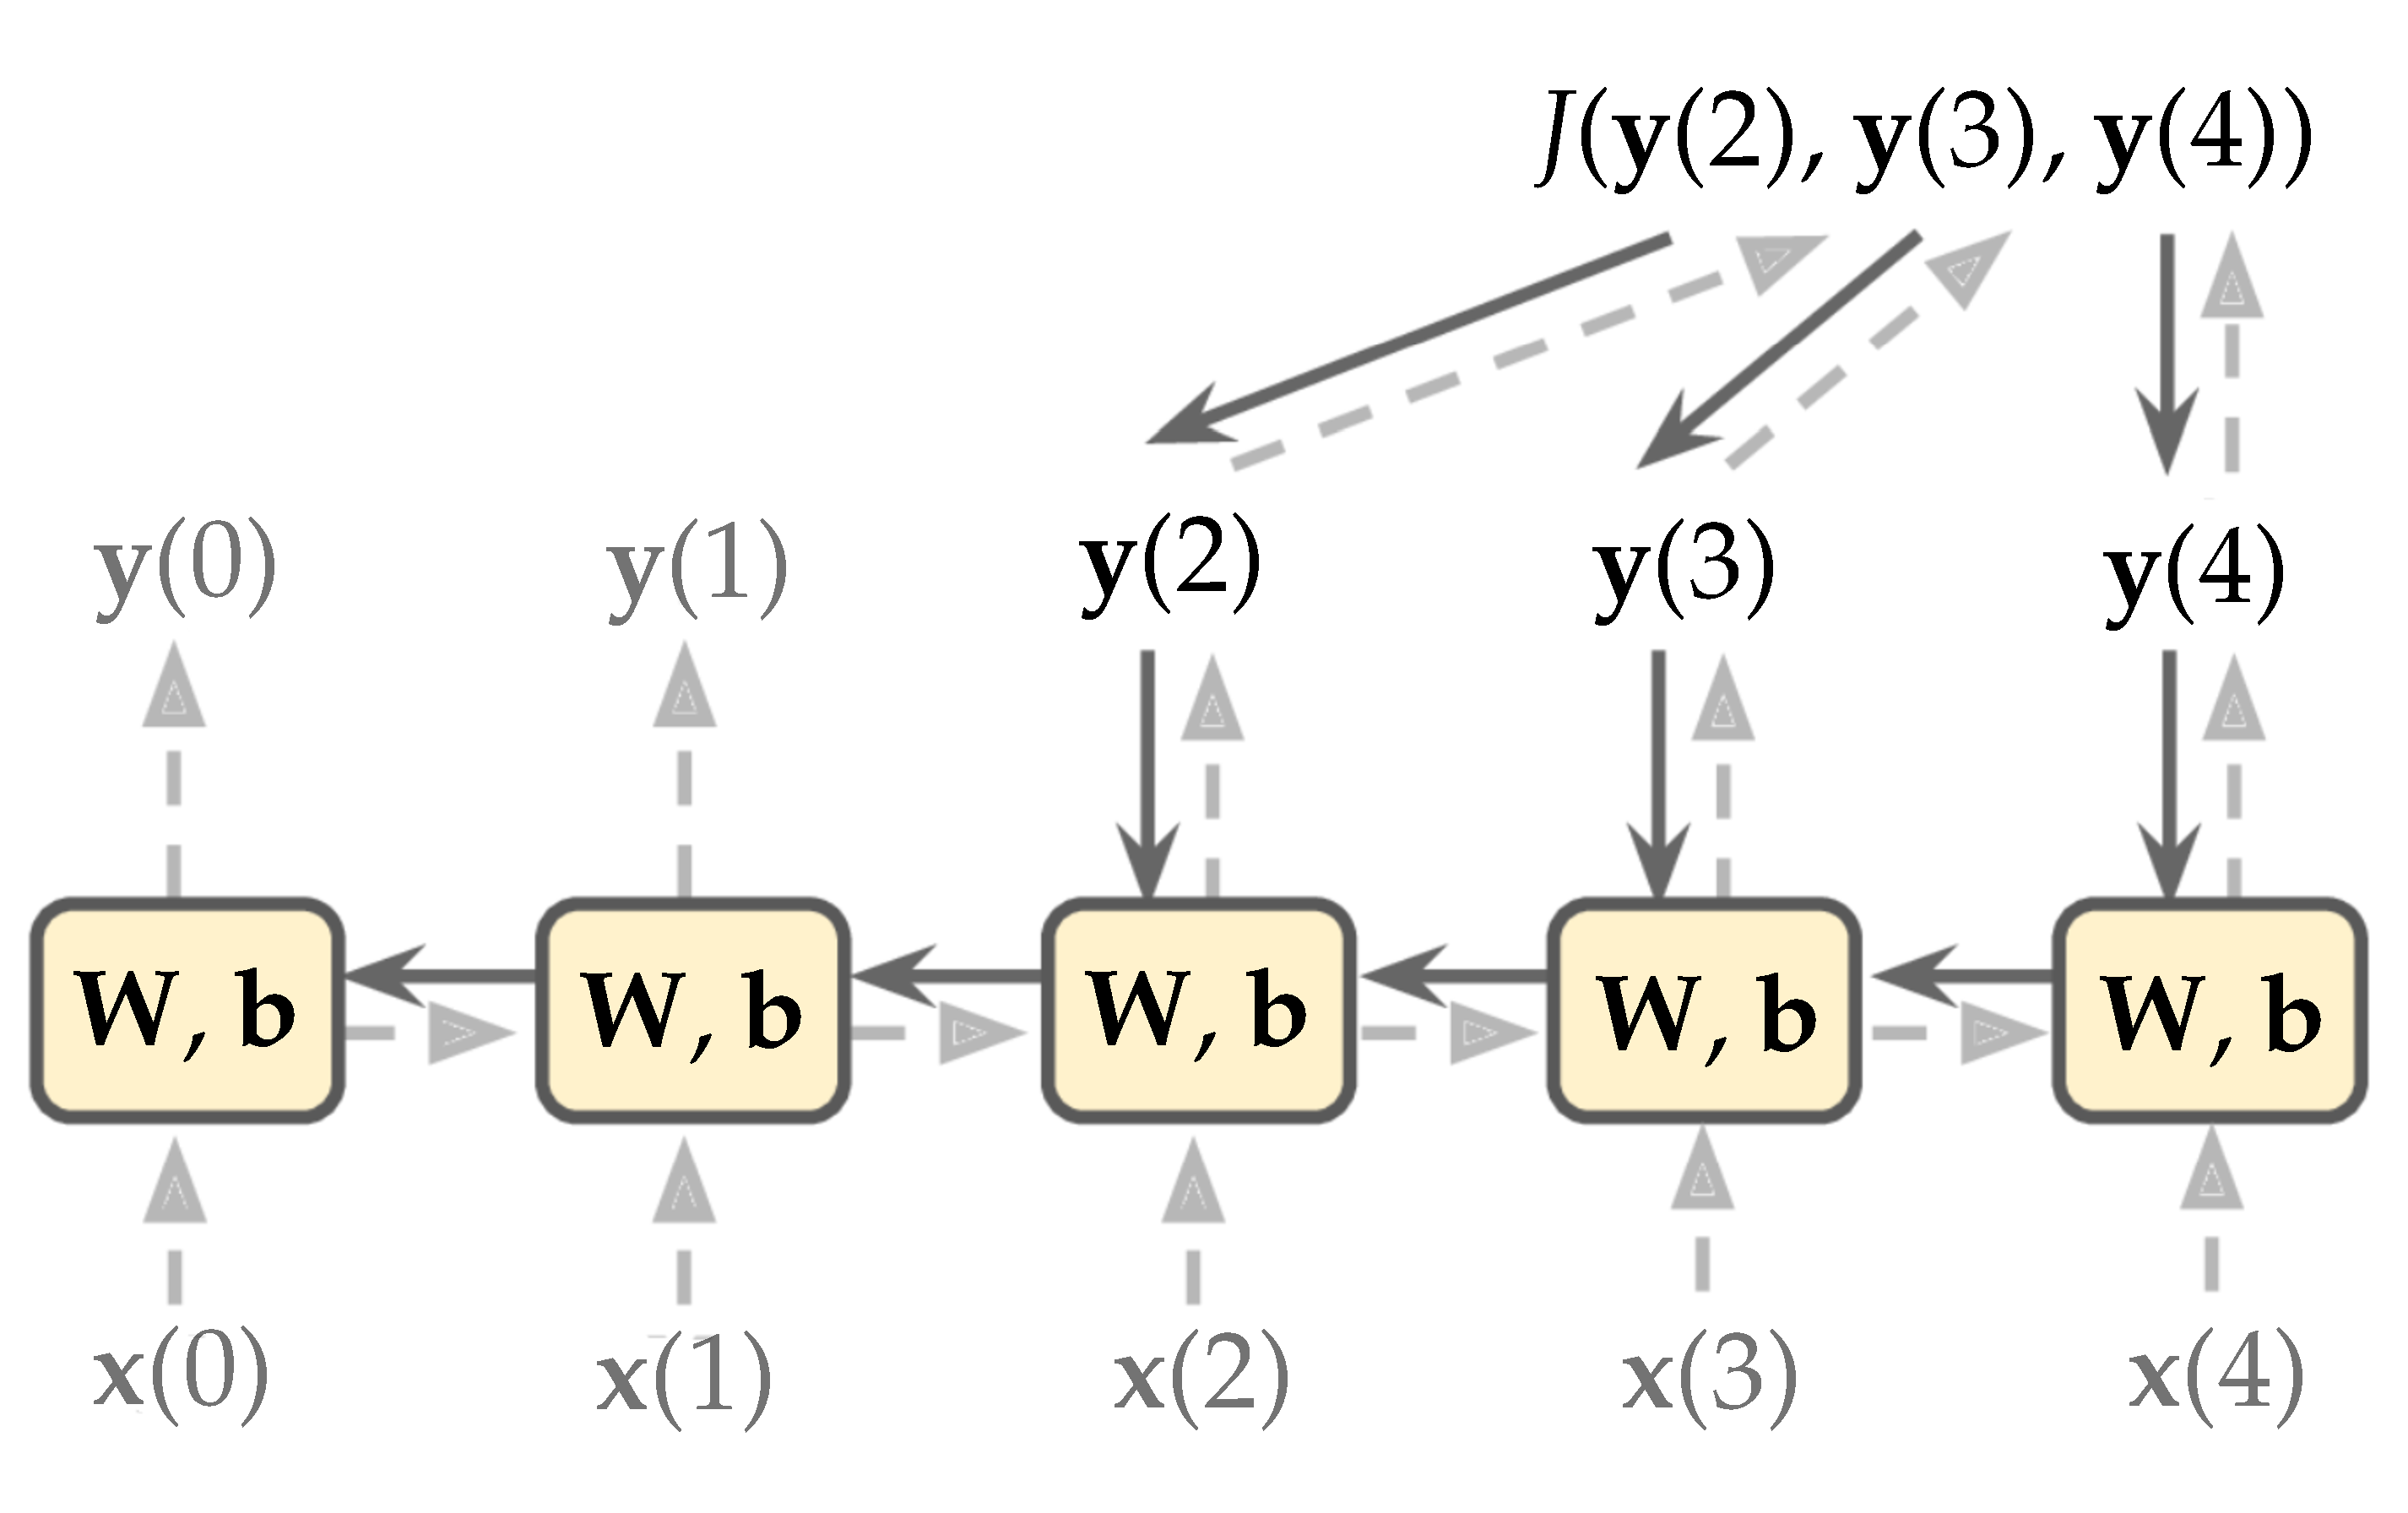
\includegraphics[scale = 0.3]{rnn-backpropagation.pdf}
\caption{Retropropagação do erro através do tempo (figura adaptada de \cite{geron2019hands})}
\label{fig:rnn-backpropagation}
\end{figure}

Logo, o algoritmo calcula a função custo $J$, considerando as saídas relevantes, e os gradientes dessa função para os pesos $\mathbf{W}$ e $\mathbf{b}$ são propagados em direção aos instantes de tempo anteriores (ignorando os instantes com saídas irrelevantes) e, como esses pesos são os mesmos em todas as camadas da rede desdobrada, eles são ajustados combinando a direção do gradiente calculado em cada instante de tempo. Este processo sintetiza a essência da retropropagação do erro através do tempo.

É importante mencionar que essa técnica também está sujeita a obstáculos semelhantes aos mencionados anteriormente sobre a retropropagação do erro tradicional, como gradientes explosivos e/ou desvanecimento dos mesmos. Além disso, como a rede recorrente é um sistema dinâmico, podem ocorrer problemas com relação à instabilidade do processo de treinamento. 

Para mitigar esses problemas, são utilizadas técnicas de \textit{gradient clipping} e normalizações \cite{geron2019hands}, além do uso de funções de ativação baseadas nas funções tangente hiperbólica ($\tanh$) e logística ($\sigmoid$), devido às saturações das mesmas para entradas muito grandes, ou muito pequenas (Figura \ref{fig:mlp-activations}).

A célula recorrente apresentada aqui é bem básica, aprendendo apenas padrões curtos. Assim, na seção seguinte apresentaremos a rede recorrente LSTM, que possui uma estrutura mais elaborada e é capaz de aprender padrões temporais mais complexos.

\subsubsection{Redes \textit{Long Short-term Memory} (LSTM)}

Devido às transformações que uma rede recorrente convencional aplica em uma entrada, parte da informação original transmitida é perdida e, depois de várias iterações, não sobra traços das primeiras entradas.

As redes LSTM (do inglês, \textit{Long Short-term Memory}) contornam esse problema inserindo portas dentro da célula recorrente que controlam o fluxo de informação \cite{greff2016lstm}.

O neurônio da rede LSTM é bem semelhante ao neurônio básico da rede recorrente mostrado anteriormente. A diferença é a presença de um vetor de longo prazo $\mathbf{c}$ e um vetor de curto prazo $\mathbf{h}$, conforme indicado na Figura \ref{fig:lstm}.

\noindent{
\begin{figure}[!ht]
\begin{center}
\begin{tikzpicture}[
    % GLOBAL CFG
    font=\sf \scriptsize,
    >=LaTeX,
    % Styles
    cell/.style={% For the main box
        rectangle, 
        rounded corners=5mm, 
        draw,
        very thick,
        },
    operator/.style={%For operators like +  and  x
        circle,
        draw,
        inner sep=-0.5pt,
        minimum height =.2cm,
        },
    function/.style={%For functions
        ellipse,
        draw,
        inner sep=1pt
        },
    ct/.style={% For external inputs and outputs
        circle,
        draw,
        line width = .75pt,
        minimum width=1cm,
        inner sep=1pt,
        },
    gt/.style={% For internal inputs
        rectangle,
        draw,
        minimum width=4mm,
        minimum height=3mm,
        inner sep=1pt
        },
    mylabel/.style={% something new that I have learned
        font=\scriptsize\sffamily
        },
    ArrowC1/.style={% Arrows with rounded corners
        rounded corners=.25cm,
        thick,
        },
    ArrowC2/.style={% Arrows with big rounded corners
        rounded corners=.5cm,
        thick,
        },
    scale = 0.95
    ]

%Start drawing the thing...    
    % Draw the cell: 
    \node [cell, minimum height =4cm, minimum width=6cm] at (0,0){} ;

    % Draw inputs named ibox#
    \node [gt] (ibox1) at (-2,-0.75) {$\sigma$};
    \node [gt] (ibox2) at (-1.5,-0.75) {$\sigma$};
    \node [gt, minimum width=1cm] (ibox3) at (-0.5,-0.75) {$\tanh$};
    \node [gt] (ibox4) at (0.5,-0.75) {$\sigma$};

   % Draw opérators   named mux# , add# and func#
    \node [operator] (mux1) at (-2,1.5) {$\times$};
    \node [operator] (add1) at (-0.5,1.5) {+};
    \node [operator] (mux2) at (-0.5,0) {$\times$};
    \node [operator] (mux3) at (1.5,0) {$\times$};
    \node [function] (func1) at (1.5,0.75) {$\tanh$};

    % Draw External inputs? named as basis c,h,x
    \node[] (c) at (-4,1.5) {$\mathbf{c}(t-1)$};
    \node[] (h) at (-4,-1.5) {$\mathbf{h}(t-1)$};
    \node[] (x) at (-2.5,-3) {$\mathbf{x}(t)$};

    % Draw External outputs? named as basis c2,h2,x2
    \node[] (c2) at (4,1.5) {$\mathbf{c}(t)$};
    \node[] (h2) at (4,-1.5) {$\mathbf{h}(t)$};
    \node[] (x2) at (2.5,3) {$\mathbf{y}(t)$};
    
    % Draw internals functions, named as basis fi,ii,ci,oi
    \node[] (fi) at (-2.35,-0.25) {$\mathbf{f}(t)$};
    \node[] (ii) at (-1.5,0.2) {$\mathbf{i}(t)$};
    \node[] (ci) at (-0.1,-0.35) {$\tilde{\mathbf{c}}(t)$};
	\node[] (oi) at (0.5,0.2) {$\mathbf{o}(t)$};      
    
% Start connecting all.
    %Intersections and displacements are used. 
    % Drawing arrows    
    \draw [ArrowC1] (c) -- (mux1) -- (add1) -- (c2);

    % Inputs
    \draw [ArrowC2] (h) -| (ibox4);
    \draw [ArrowC1] (h -| ibox1)++(-0.5,0) -| (ibox1); 
    \draw [ArrowC1] (h -| ibox2)++(-0.5,0) -| (ibox2);
    \draw [ArrowC1] (h -| ibox3)++(-0.5,0) -| (ibox3);
    \draw [ArrowC1] (x) -- (x |- h)-| (ibox3);

    % Internal
    \draw [->, ArrowC2] (ibox1) -- (mux1);
    \draw [->, ArrowC2] (ibox2) |- (mux2);
    \draw [->, ArrowC2] (ibox3) -- (mux2);
    \draw [->, ArrowC2] (ibox4) |- (mux3);
    \draw [->, ArrowC2] (mux2) -- (add1);
    \draw [->, ArrowC1] (add1 -| func1)++(-0.5,0) -| (func1);
    \draw [->, ArrowC2] (func1) -- (mux3);

    %Outputs
    \draw [->, ArrowC2] (mux3) |- (h2);
    \draw [->] (add1) |- (c2);
    \draw (c2 -| x2) ++(0,-0.1) coordinate (i1);
    \draw [-, ArrowC2] (h2 -| x2)++(-0.5,0) -| (i1);
    \draw [->, ArrowC2] (i1)++(0,0.2) -- (x2);

\end{tikzpicture}
\caption{Estrutura interna de uma célula LSTM}
\label{fig:lstm}
\end{center}
\end{figure}
}

Durante o processo de treinamento, a rede aprende o que deve ser armazenado no vetor $\mathbf{c}(t)$ e, do que foi guardado, o que deve ser descartado e o que deve ser levado em conta na hora de estimar a próxima saída.

A primeira operação realizada nesse vetor é a multiplicação elemento a elemento ($\otimes$) com o vetor $\mathbf{f}(t)$. Essa operação também é chamada de porta do esquecimento (do inglês, \textit{forget gate}) pois ela determina quais elementos de $\mathbf{c}(t-1)$ serão descartados, ou seja, quais memórias de instantes passados no longo prazo serão esquecidas.

Após a incorporação de novas informações na operação de soma elemento a elemento ($\oplus$), o vetor $\mathbf{c}(t-1)$ é mandado para a saída da célula e uma cópia sua passa pela função tangente hiperbólica e é filtrado pela porta de saída (do inglês, \textit{output gate}), formando o vetor de curto prazo $\mathbf{h}(t)$, que é também a saída $\mathbf{y}(t)$.

A entrada do neurônio LSTM, além de incluir o vetor $\mathbf{c}(t)$, também inclui os vetores $\mathbf{h}(t-1)$ e $\mathbf{x}(t)$. A partir destas informações, são gerados os vetores $\mathbf{f}(t)$, $\mathbf{i}(t)$, $\tilde{\mathbf{c}}(t)$ e $\mathbf{o}(t)$.

Perceba que o vetor $\tilde{\mathbf{c}}(t)$ é a saída de uma célula recorrente básica, considerando a tangente hiperbólica como função de ativação. Ou seja, ela é composta pela ponderação entre os estados anteriores de curto prazo $\mathbf{h}(t)$ e a entrada atual $\mathbf{x}(t)$, além do vetor de \textit{bias} $\mathbf{b}(t)$. A LSTM guarda as partes mais relevantes do vetor $\tilde{\mathbf{c}}(t)$ no vetor $\mathbf{c}(t-1)$ através da soma elemento a elemento mencionada anteriormente.

Os outros vetores restantes representam operações de controle do fluxo de informação dentro do neurônio, cada termo variando de $0$ a $1$ devido à função logística ($\sigma$). Assim, ao serem multiplicadas elemento a elemento, controlam quais informações serão eliminadas.

No caso, $\mathbf{f}(t)$ controla quais partes de $\mathbf{c}(t-1)$ serão apagadas, $\mathbf{i}(t)$ controla quais informações de $\tilde{\mathbf{c}}(t)$ serão agregadas ao vetor $\mathbf{c}(t-1)$ e o vetor $\mathbf{o}(t)$ controla quais componentes de $\mathbf{c}(t-1)$ deverão formar a saída $\mathbf{y}(t)$ e o vetor de curto prazo $\mathbf{h}(t)$.

O conjunto de equações abaixo mostra as operações presentes na estrutura interna da célula LSTM, assim como a saída para o instante $t$, denotada por $\mathbf{y}(t)$:
\begin{subequations}
\begin{equation}
\mathbf{f}(t) = \sigma(\mathbf{W}_f [\mathbf{h}(t-1), \mathbf{x}(t)] + \mathbf{b}_f)
\end{equation}
\begin{equation}
\mathbf{i}(t) = \sigma(\mathbf{W}_i [\mathbf{h}(t-1), \mathbf{x}(t)] + \mathbf{b}_i)
\end{equation}
\begin{equation}
\tilde{\mathbf{c}}(t) = \tanh(\mathbf{W}_c [\mathbf{h}(t-1), \mathbf{x}(t)] + \mathbf{b}_c)
\end{equation}
\begin{equation}
\mathbf{c}(t) = \mathbf{f}(t) \otimes \mathbf{c}(t-1) + \mathbf{i}(t) \otimes \tilde{\mathbf{c}}(t)
\end{equation}
\begin{equation}
\mathbf{o}(t) = \sigma(\mathbf{W}_o [\mathbf{h}(t-1), \mathbf{x}(t)] + \mathbf{b}_o)
\end{equation}
\begin{equation}
\mathbf{y}(t) = \mathbf{h}(t) = \mathbf{o}(t) \otimes \tanh (\mathbf{c}(t))
\end{equation}
\end{subequations}

À semelhança das redes recorrentes convencionais, o treinamento de uma LSTM também é realizado através de algoritmos de otimização baseados em derivadas da função custo propagadas ao longo da estrutura e ao longo do tempo, utilizando o algoritmo BPTT.

Resumidamente, as LSTMs manipulam o vetor de longo prazo $\mathbf{c}(t)$, aprendendo durante o treinamento o que deve ser guardado nele, o que deve ser descartado e o que deve ser aproveitado para gerar a saída $\mathbf{y}(t)$ e o vetor de curto prazo $\mathbf{h}(t)$. Dessa forma, podemos dizer que a atualização do vetor de estados $\mathbf{c}(t)$ é feita com o descarte de informações e a incorporação de novidades vindas da entrada.

Depois de uma exposição sobre os modelos preditores que utilizaremos nessa pesquisa, concluiremos este relatório com a indicação dos próximos passos do estudo, já definindo quais são os sistemas caóticos que analisaremos com as redes neurais artificiais citadas.

\section{Próximos Passos}

Como nessa primeira parte da iniciação o foco foi uma pesquisa bibliográfica dos temas a serem estudados nela, a segunda metade será voltada para a aplicação em si da predição das séries temporais de sistemas caóticos.

Para os experimentos computacionais, optamos pelas séries temporais associadas ao  mapa logístico, descrito pelo cientista Robert May \cite{may1976simple}, ao mapa de Hénon, apresentado pelo astrônomo e matemático francês Michel Hénon \cite{henon1976two}, ao sistema de Mackey-Glass, dos cientistas Michael Mackey e Leon Glass \cite{mackey1977oscillation}, e ao clássico sistema de Lorenz, um dos  mais incríveis e fundamentais trabalhos de sistemas caóticos, introduzido pelo matemático e meteorologista Edward Norton Lorenz \cite{lorenz1963deterministic}. Este grupo de séries foi selecionado com o intuito de criar cenários diversificados para a análise do comportamento das diferentes redes neurais, considerando sistemas a tempo contínuo (Lorenz e Mackey-Glass) e sistemas a tempo discreto (mapa de Hénon e mapa logístico). 

Em seguida, determinaremos aspectos mais fundamentais das redes neurais que serão utilizadas, como, por exemplo, a arquitetura empregada, assim como as métricas para o treinamento e análise. Para essa etapa, também planejamos um estudo das redes GRU (do inglês \textit{Gated Recurrent Unit}) \cite{cho2014learning} e ESN (do inglês \textit{Echo State Network}) \cite{jaeger2007echo}, sendo que a última, em outros trabalhos de pesquisa, já indicou um bom desempenho preliminar no contexto de predição de séries temporais originadas por sistemas caóticos \cite{boccato2013novas}.

Após isso, faremos a aplicação das redes neurais à predição das séries escolhidas, avaliando a sensibilidade paramétrica de cada estrutura na busca das melhores configurações, a fim de traçar um quadro comparativo entre as técnicas consideradas. 

Por fim, compilaremos os resultados no relatório final, de forma a conter uma discussão ampla e representativa dos ensaios realizados e das conclusões obtidas. 

\bibliographystyle{ieeetr}

\bibliography{bib}

\pdfinfo{
   /Title  (Relatório EE015 - João Pedro O. Pagnan)
   /CreationDate (D:20040502195600)
}

\end{document}